\documentclass[10pt, compress]{beamer}

\usetheme[numbering=fraction, progressbar=none, titleformat=smallcaps, sectionpage=none]{metropolis}

\usepackage{sourcecodepro}
\usepackage{booktabs}
\usepackage{array}
\usepackage{listings}
\usepackage{graphicx}
\usepackage[brazilian]{babel}
\usepackage[scale=2]{ccicons}
\usepackage{url}
\usepackage{relsize}
\usepackage{wasysym}

\setsansfont[BoldFont={Source Sans Pro Semibold},
              Numbers={OldStyle}]{Source Sans Pro}

\usepackage{pgfplots}
\usepgfplotslibrary{dateplot}

\definecolor{Base}{HTML}{191F26}
\definecolor{Accent}{HTML}{157FFF}

\setbeamercolor{alerted text}{fg=Accent}
\setbeamercolor{frametitle}{bg=Base}

\lstset{ %
  backgroundcolor={},
  basicstyle=\ttfamily\footnotesize,
  breakatwhitespace=true,
  breaklines=true,
  captionpos=n,
  commentstyle=\color{orange},
  escapeinside={\%*}{*)},
  extendedchars=true,
  frame=n,
  keywordstyle=\color{Accent},
  language=C++,
  rulecolor=\color{black},
  showspaces=false,
  showstringspaces=false,
  showtabs=false,
  stepnumber=2,
  stringstyle=\color{gray},
  tabsize=2,
  keywords={thrust,plus,device_vector, copy,transform,begin,end, copyin,
  copyout, acc, \_\_global\_\_, void, int, float, main, threadIdx, blockIdx,
  blockDim, if, else, malloc, NULL, cudaMalloc, cudaMemcpy, cudaSuccess,
  cudaGetLastError, cudaDeviceSynchronize, cudaFree, cudaMemcpyDeviceToHost,
  cudaMemcpyHostToDevice, const, data, independent, kernels, loop,
  fprintf, stderr, cudaGetErrorString, EXIT_FAILURE, for, dim3},
  otherkeywords={::, \#pragma, \#include, <<<,>>>, \&, \*, +, -, /, [, ], >, <}
}

\renewcommand*{\UrlFont}{\ttfamily\smaller\relax}

\graphicspath{{../img/}}

\title{FPGAs, GPUs e Xeon Phi}
\author{\footnotesize Pedro Bruel \\ {\scriptsize \emph{phrb@ime.usp.br}} \\[0.1cm] \footnotesize Marcos Amarís \\ {\scriptsize \emph{amaris@ime.usp.br}} \\[0.1cm]}
\institute{
\includegraphics[height=2cm]{imelogo}\\[0.2cm] Instituto de Matemática e Estatística \\ Universidade de São Paulo}
\date{\scriptsize 28 de Março de 2017}

\begin{document}

\maketitle

\section*{Introdução}

\subsection*{Sobre}

\begin{frame}
    \frametitle{Sobre}
    \begin{columns}[T,onlytextwidth]
        \column{0.3\textwidth}
        \begin{center}
            
\includegraphics[width=.75\textwidth]{pedro}

            Pedro Bruel \\
            \emph{\alert{phrb}@ime.usp.br} \\
        \end{center}

        \column{0.3\textwidth}
        \begin{center}
            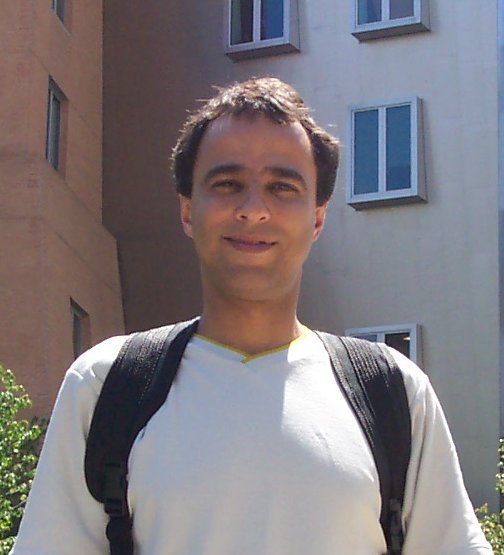
\includegraphics[width=.65\textwidth]{alfredo}

            Alfredo Goldman \\
            \emph{\alert{gold}@ime.usp.br} \\
        \end{center}

        \column{0.3\textwidth}
        \begin{center}
            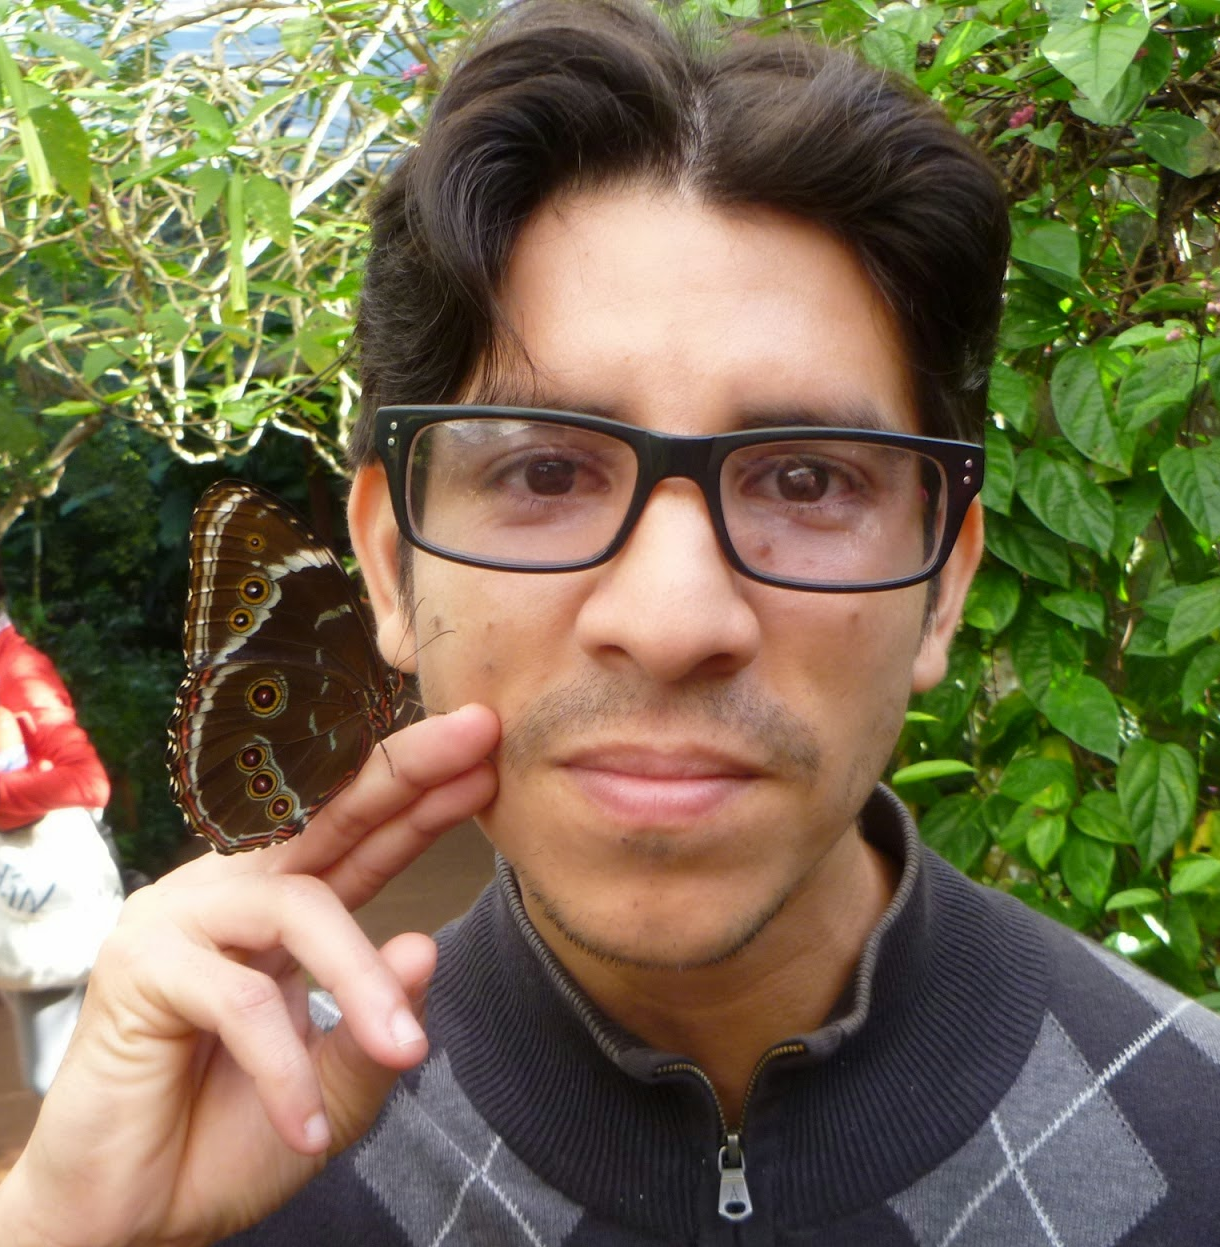
\includegraphics[width=.75\textwidth]{marcos}

            Marcos Amarís \\
            \emph{\alert{amaris}@ime.usp.br} \\
        \end{center}
    \end{columns}
\end{frame}

\subsection*{Roteiro}

\begin{frame}
    \frametitle{Roteiro}
    \setbeamertemplate{section in toc}[sections numbered]
    \tableofcontents
\end{frame}

\begin{frame}
    \frametitle{Slides}
    \begin{center}
        
\includegraphics[width=.18\textwidth]{github}
    \end{center}
    Os slides estão no \alert{GitHub}:

    \begin{itemize}
        \item \url{github.com/phrb/MAC5742-0219-fpgas-gpus-xeonphi}
    \end{itemize}
\end{frame}

\section{FPGAs}

\subsection{Computação Reconfigurável}

\begin{frame}
    \frametitle{Computação Reconfigurável}
    \begin{center}
        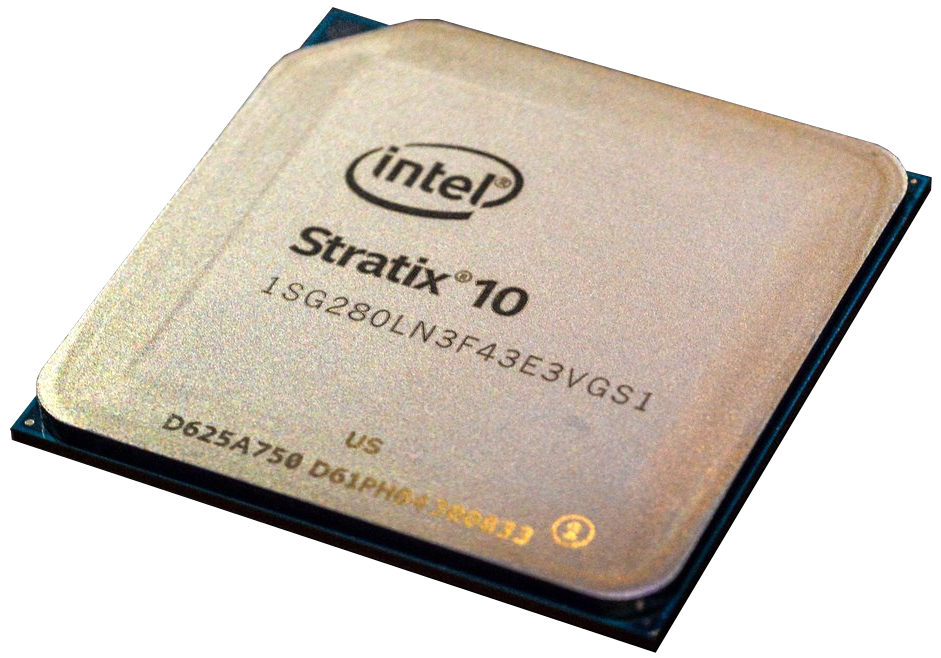
\includegraphics[width=.65\textwidth]{stratix10}
    \end{center}
\end{frame}

\begin{frame}
    \frametitle{Computação Reconfigurável}
    \alert{Field-Programmable} Gate Arrays (FPGAs):

    \begin{itemize}
        \item Dispositivos feitos de semicondutores
        \item Funcionalidade definível após fabricação
        \item \alert{Reconfiguráveis} mesmo após instalação
        \item Adaptáveis a diferentes aplicações
        \item \alert{Consumo eficiente de energia}
    \end{itemize}

    \pause
    Compostas de uma matriz de elementos lógicos (\alert{Gate Array}):

    \begin{itemize}
        \item Elementos Lógicos: Portas Lógicas, Transistores (\alert{LEs})
        \item Conexões entre LEs: \alert{Interconnect}
        \item Tabelas de Verdade: \textit{Lookup Tables} (\alert{LUTs})
        \item 2D Gate Arrays: \alert{LEs} + \alert{LUTs} + \alert{Interconnect}
    \end{itemize}
\end{frame}

\begin{frame}
    \frametitle{Programabilidade vs. Desempenho}
    \begin{center}
        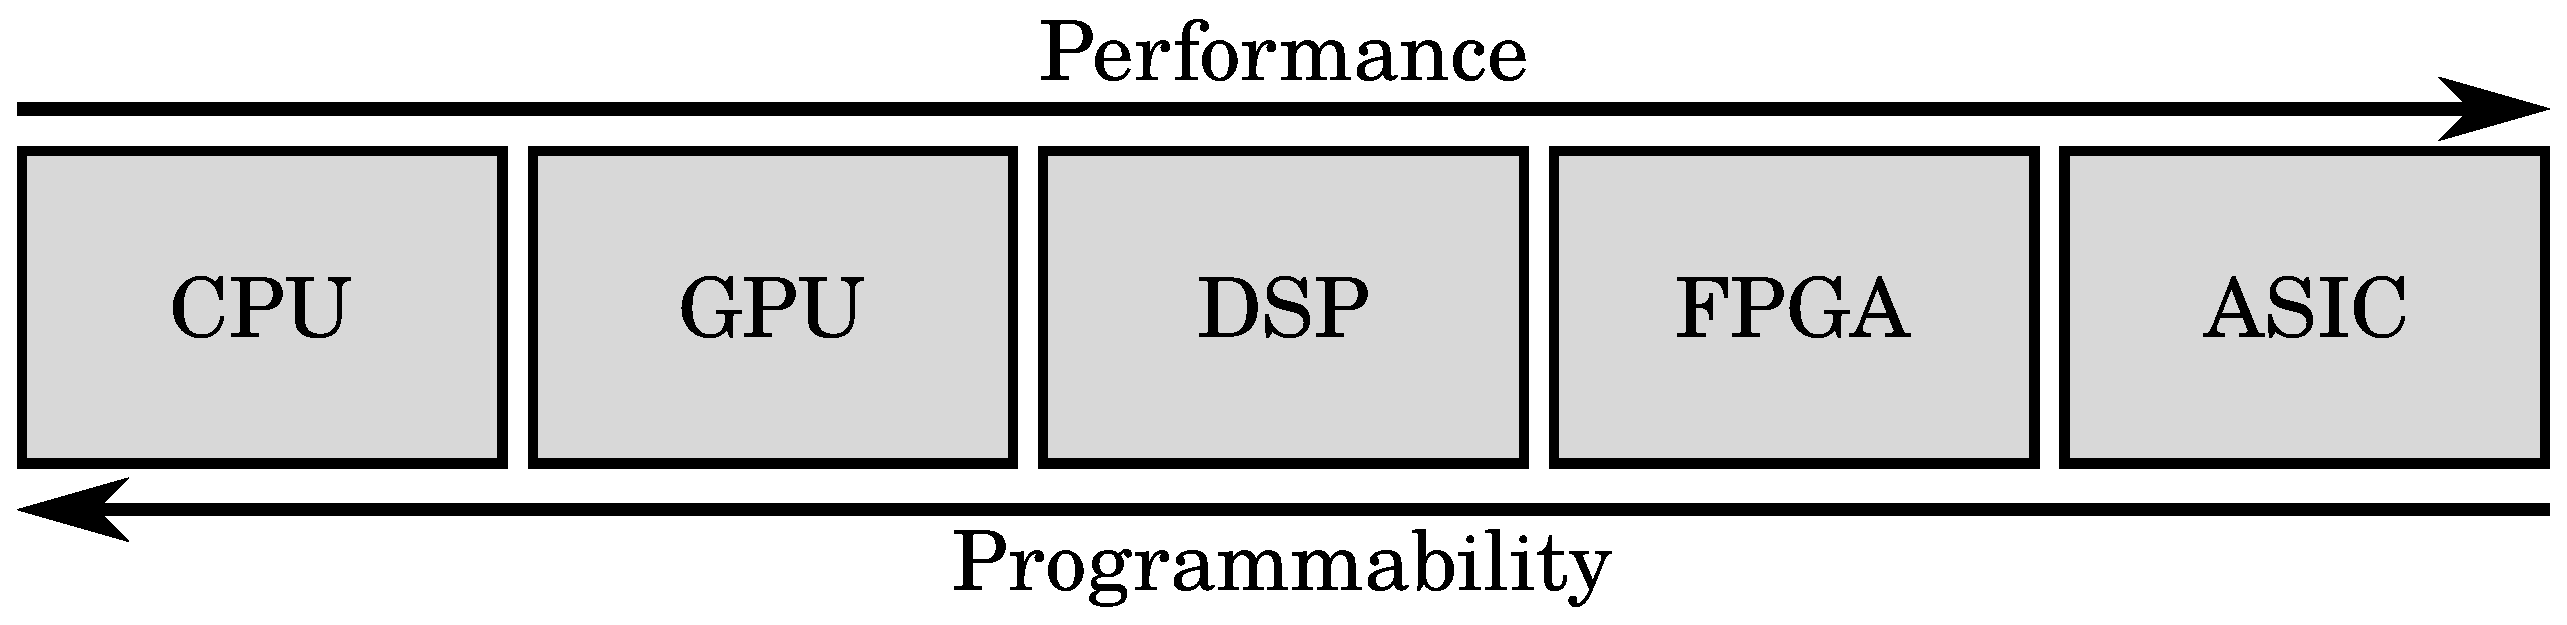
\includegraphics[width=\textwidth]{fpga-tradeoff}
    \end{center}
\end{frame}

\begin{frame}
    \frametitle{Programabilidade vs. Desempenho vs. Generalidade}
    \begin{center}
        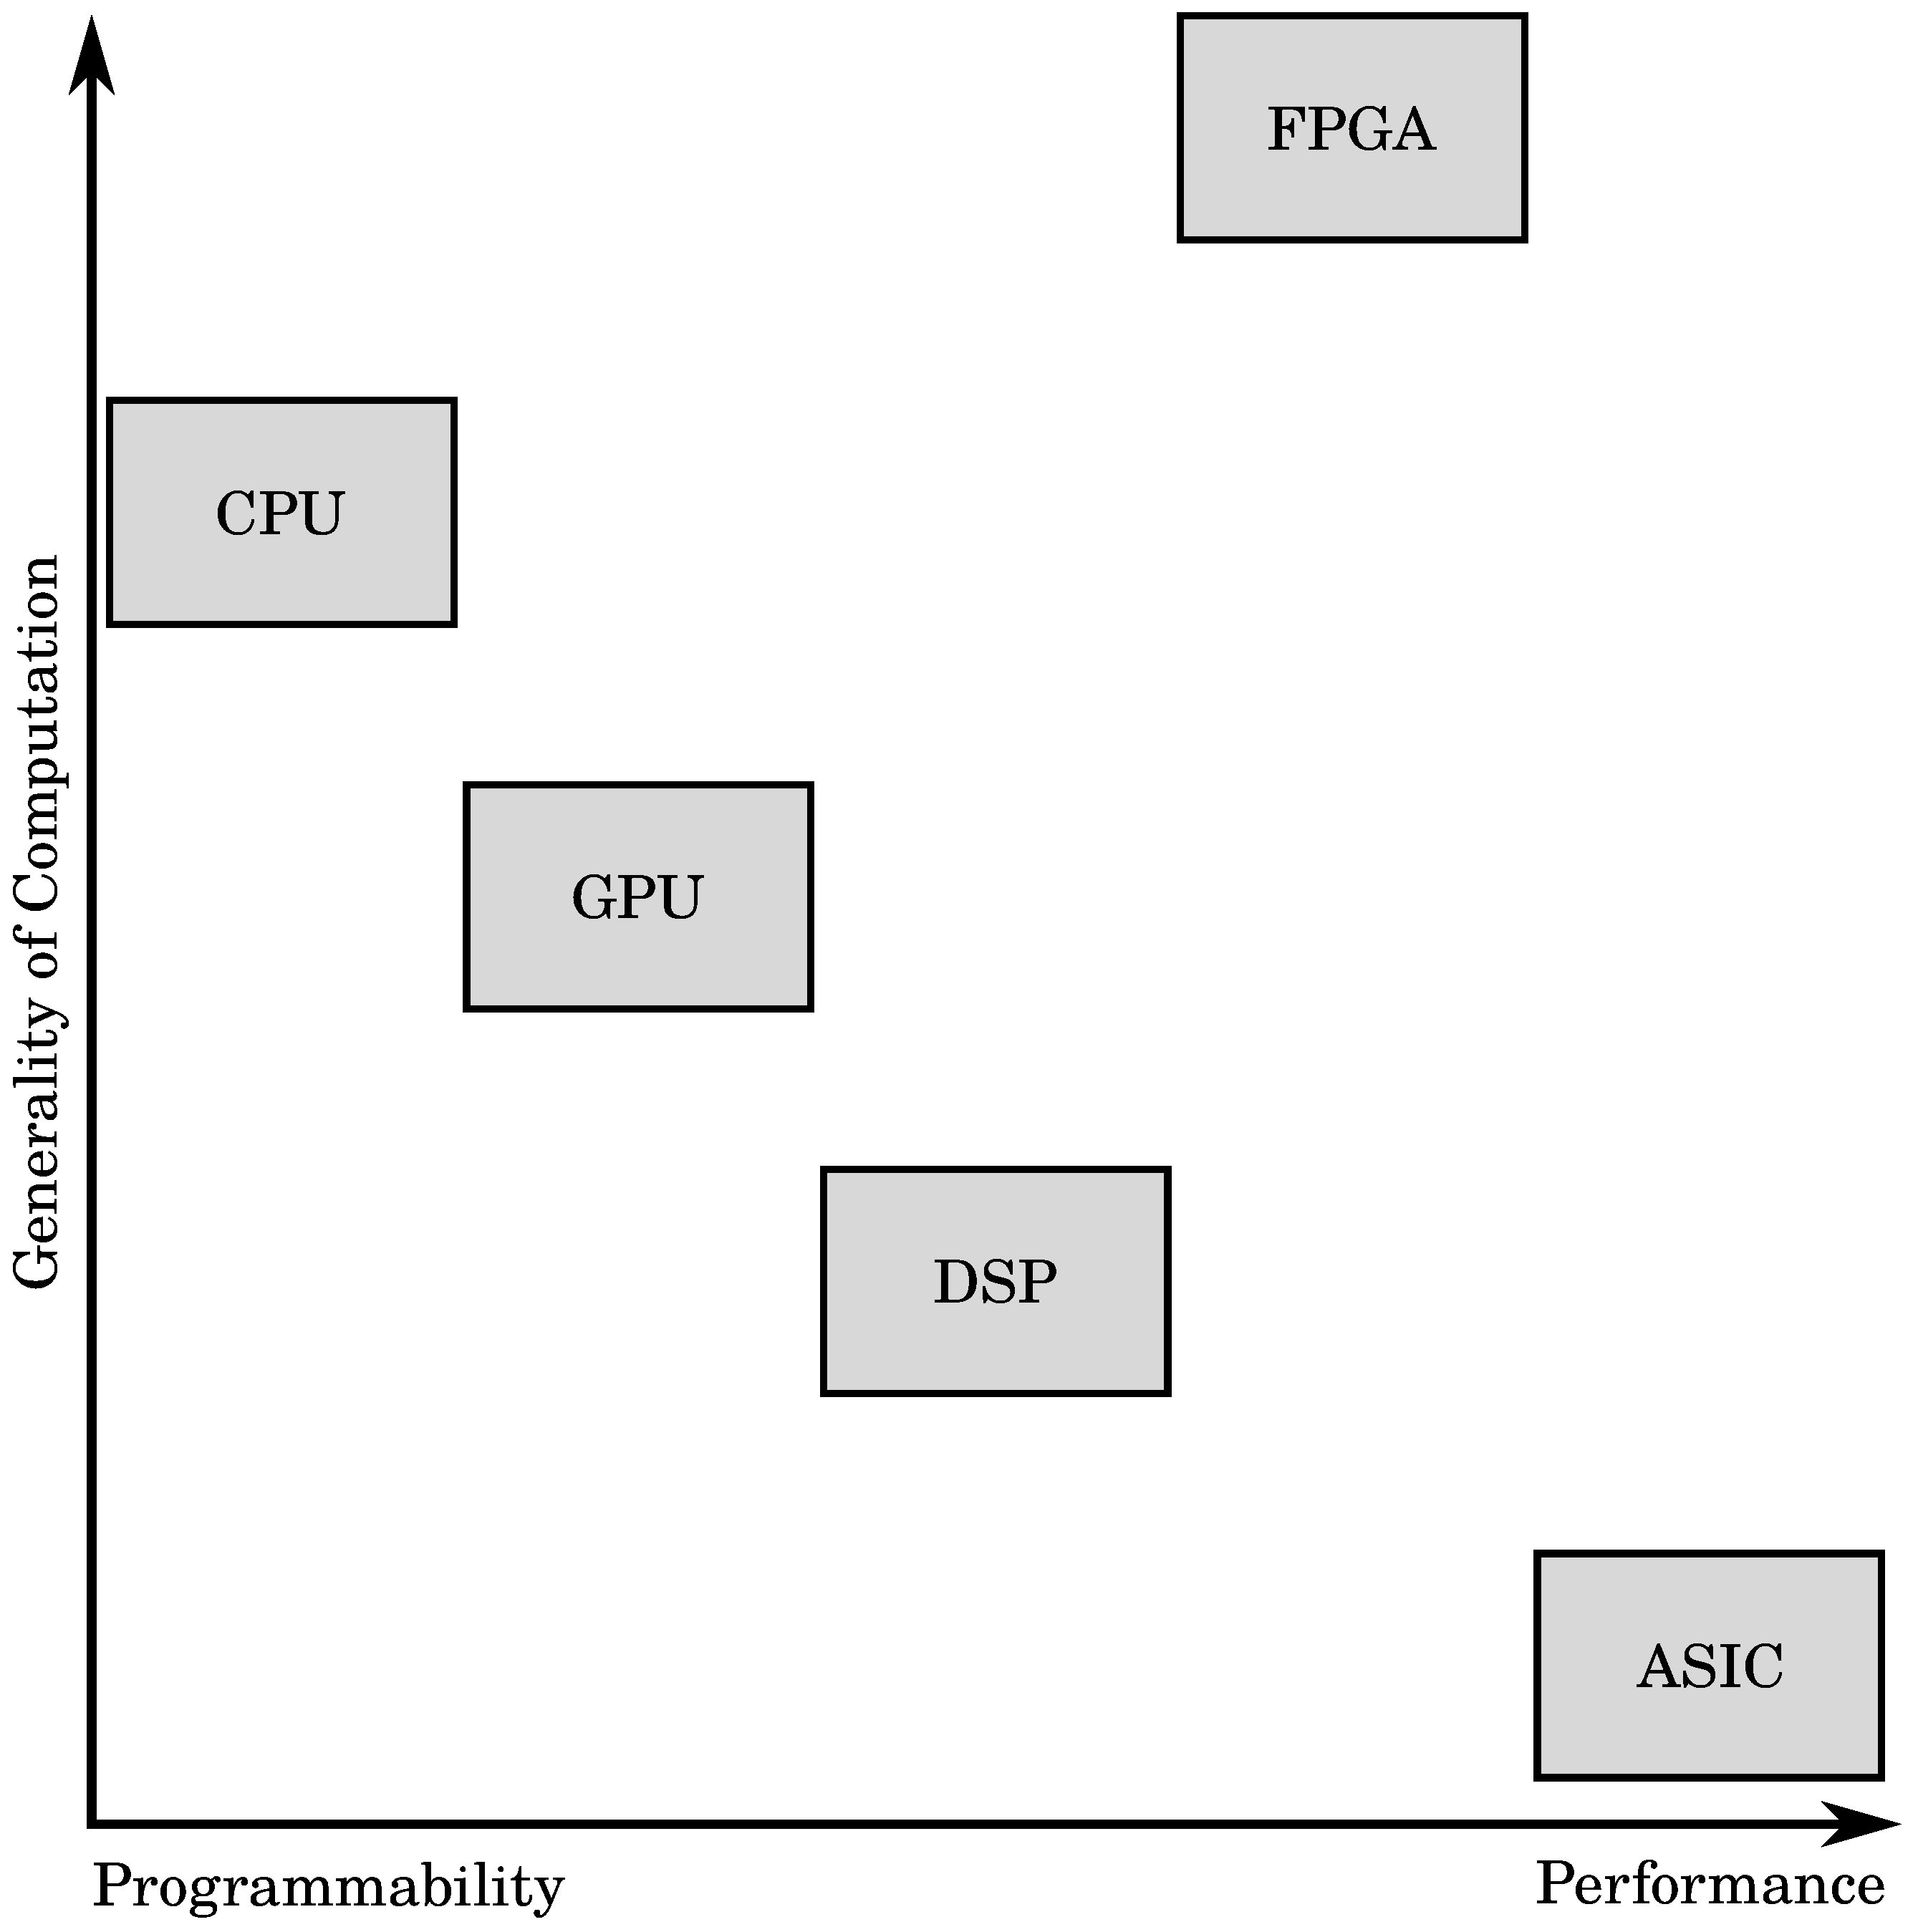
\includegraphics[width=.7\textwidth]{fpga-tradeoff-2}
    \end{center}
\end{frame}

\begin{frame}
    \frametitle{Programabilidade vs. Desempenho vs. Eficiência}
    \begin{center}
        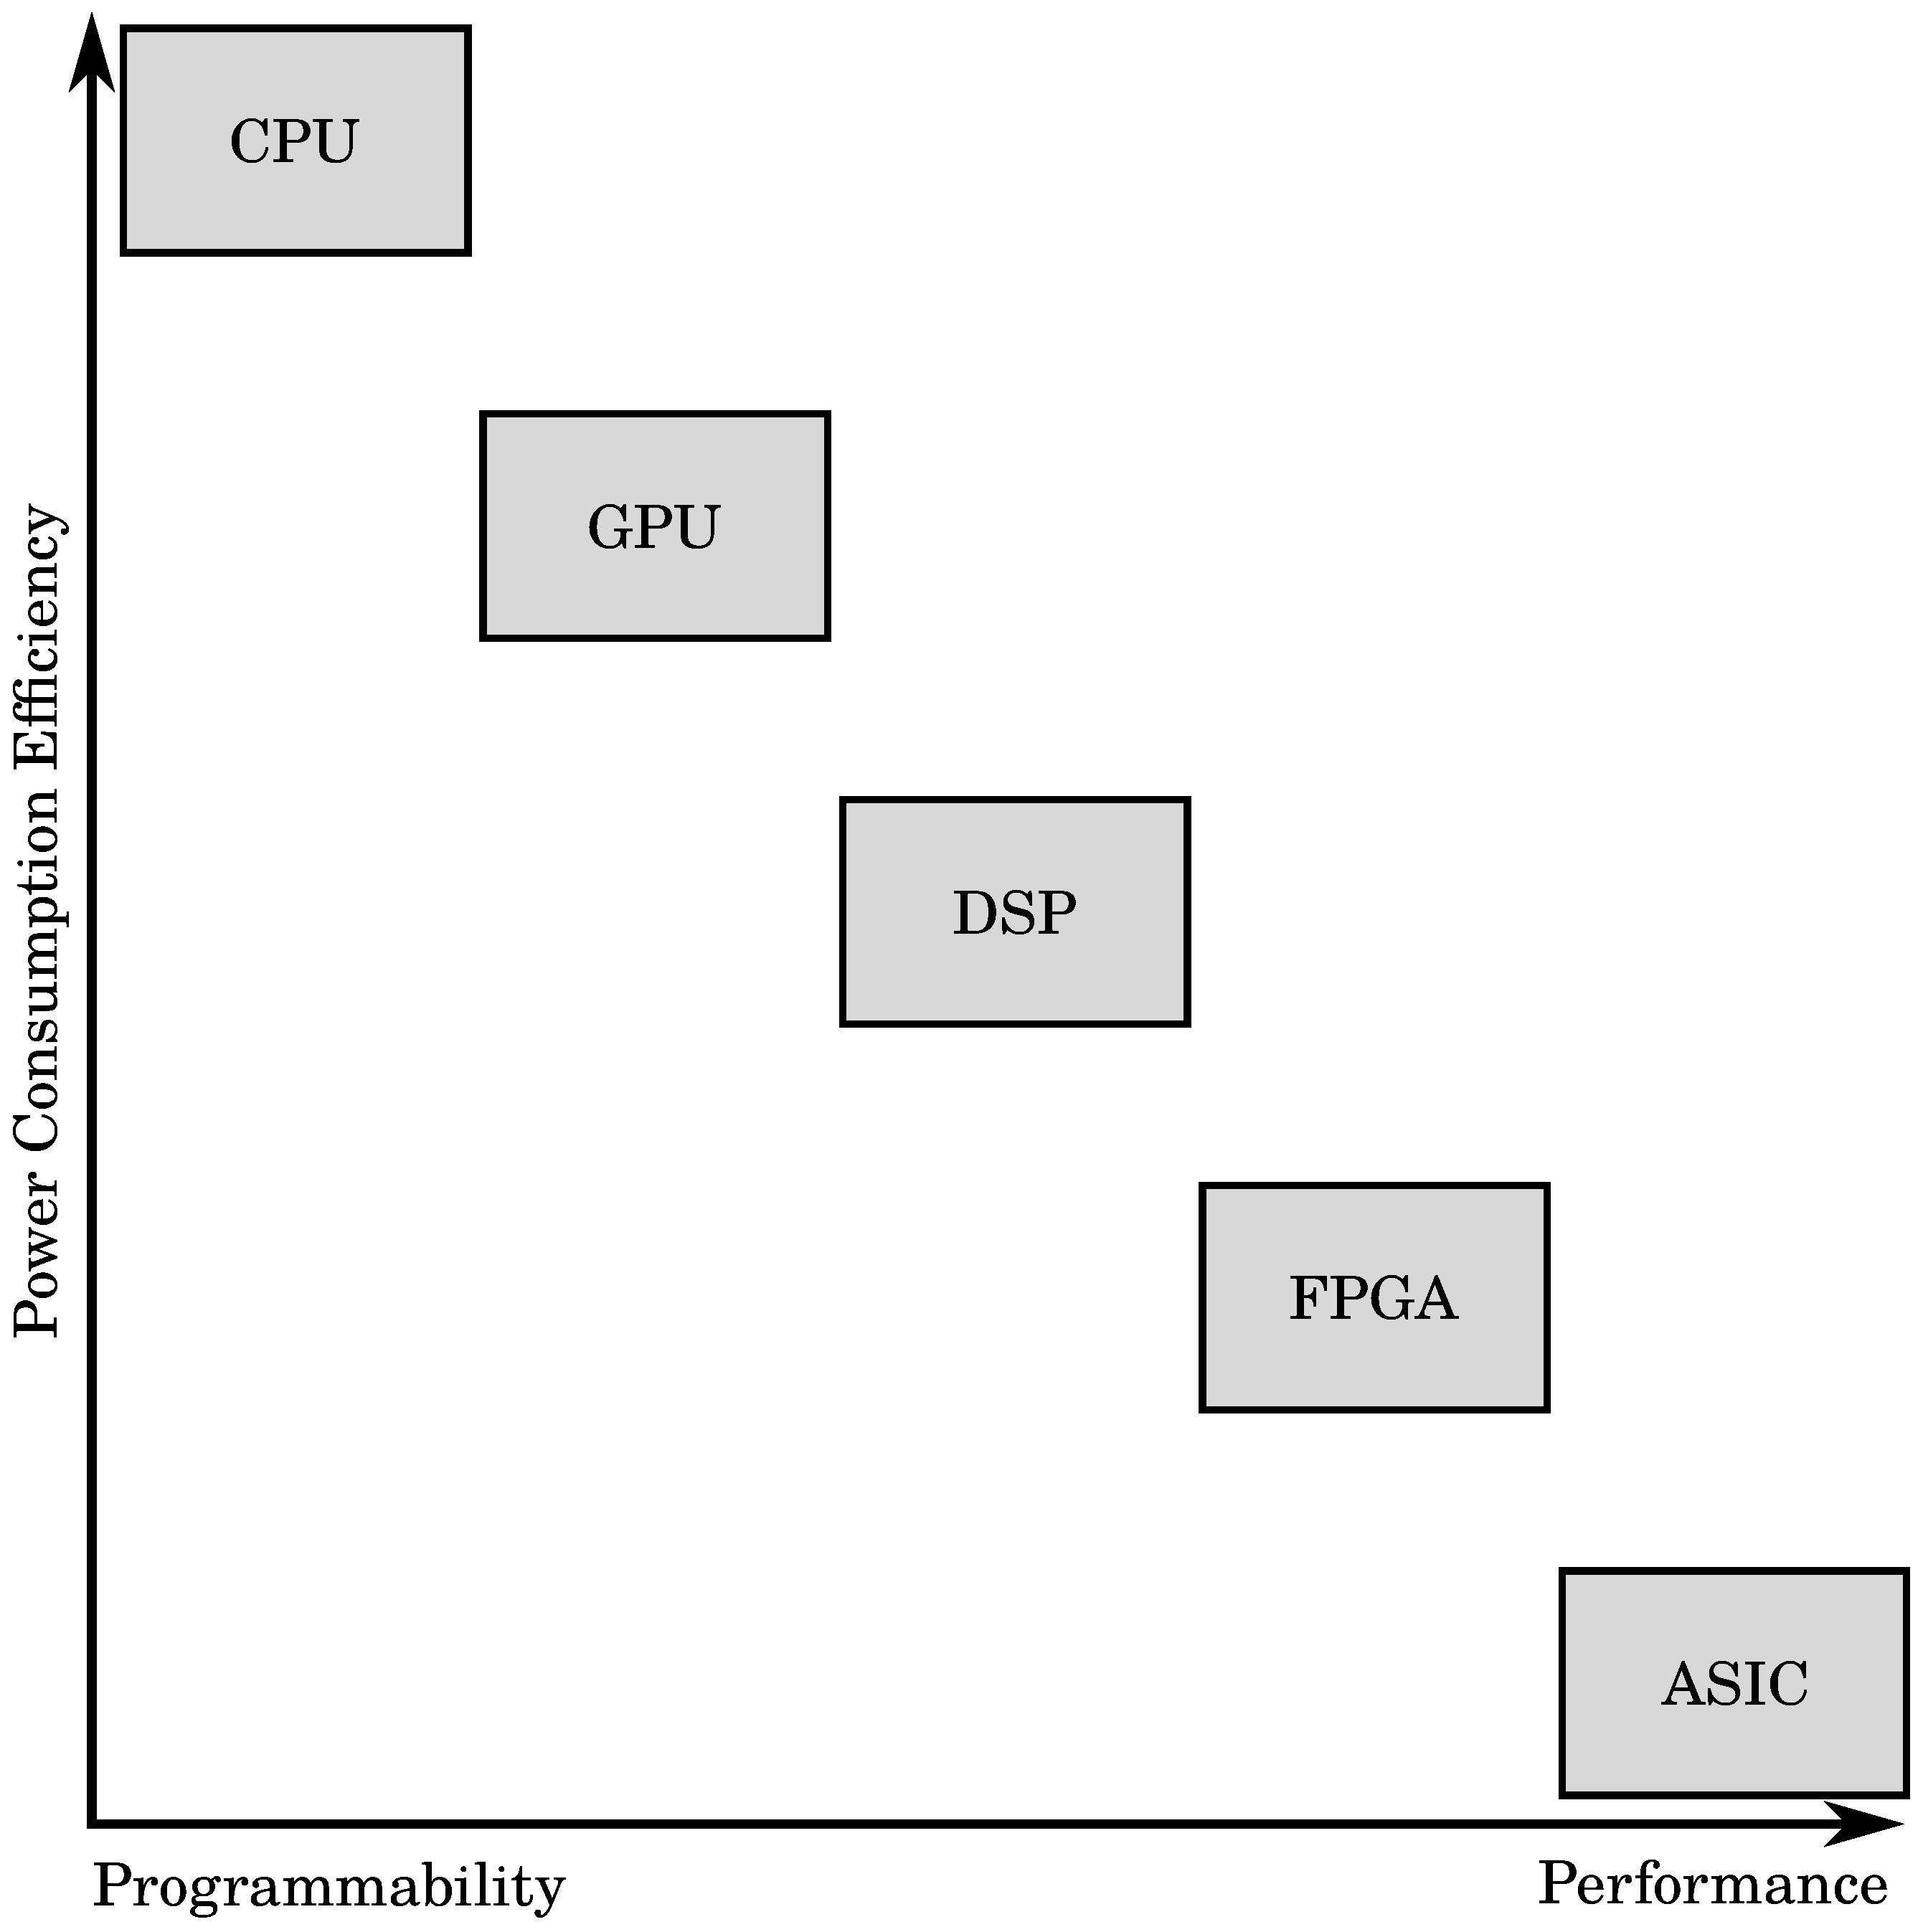
\includegraphics[width=.7\textwidth]{fpga-tradeoff-3}
    \end{center}
\end{frame}

\begin{frame}
    \frametitle{Aplicações}
    \begin{center}
        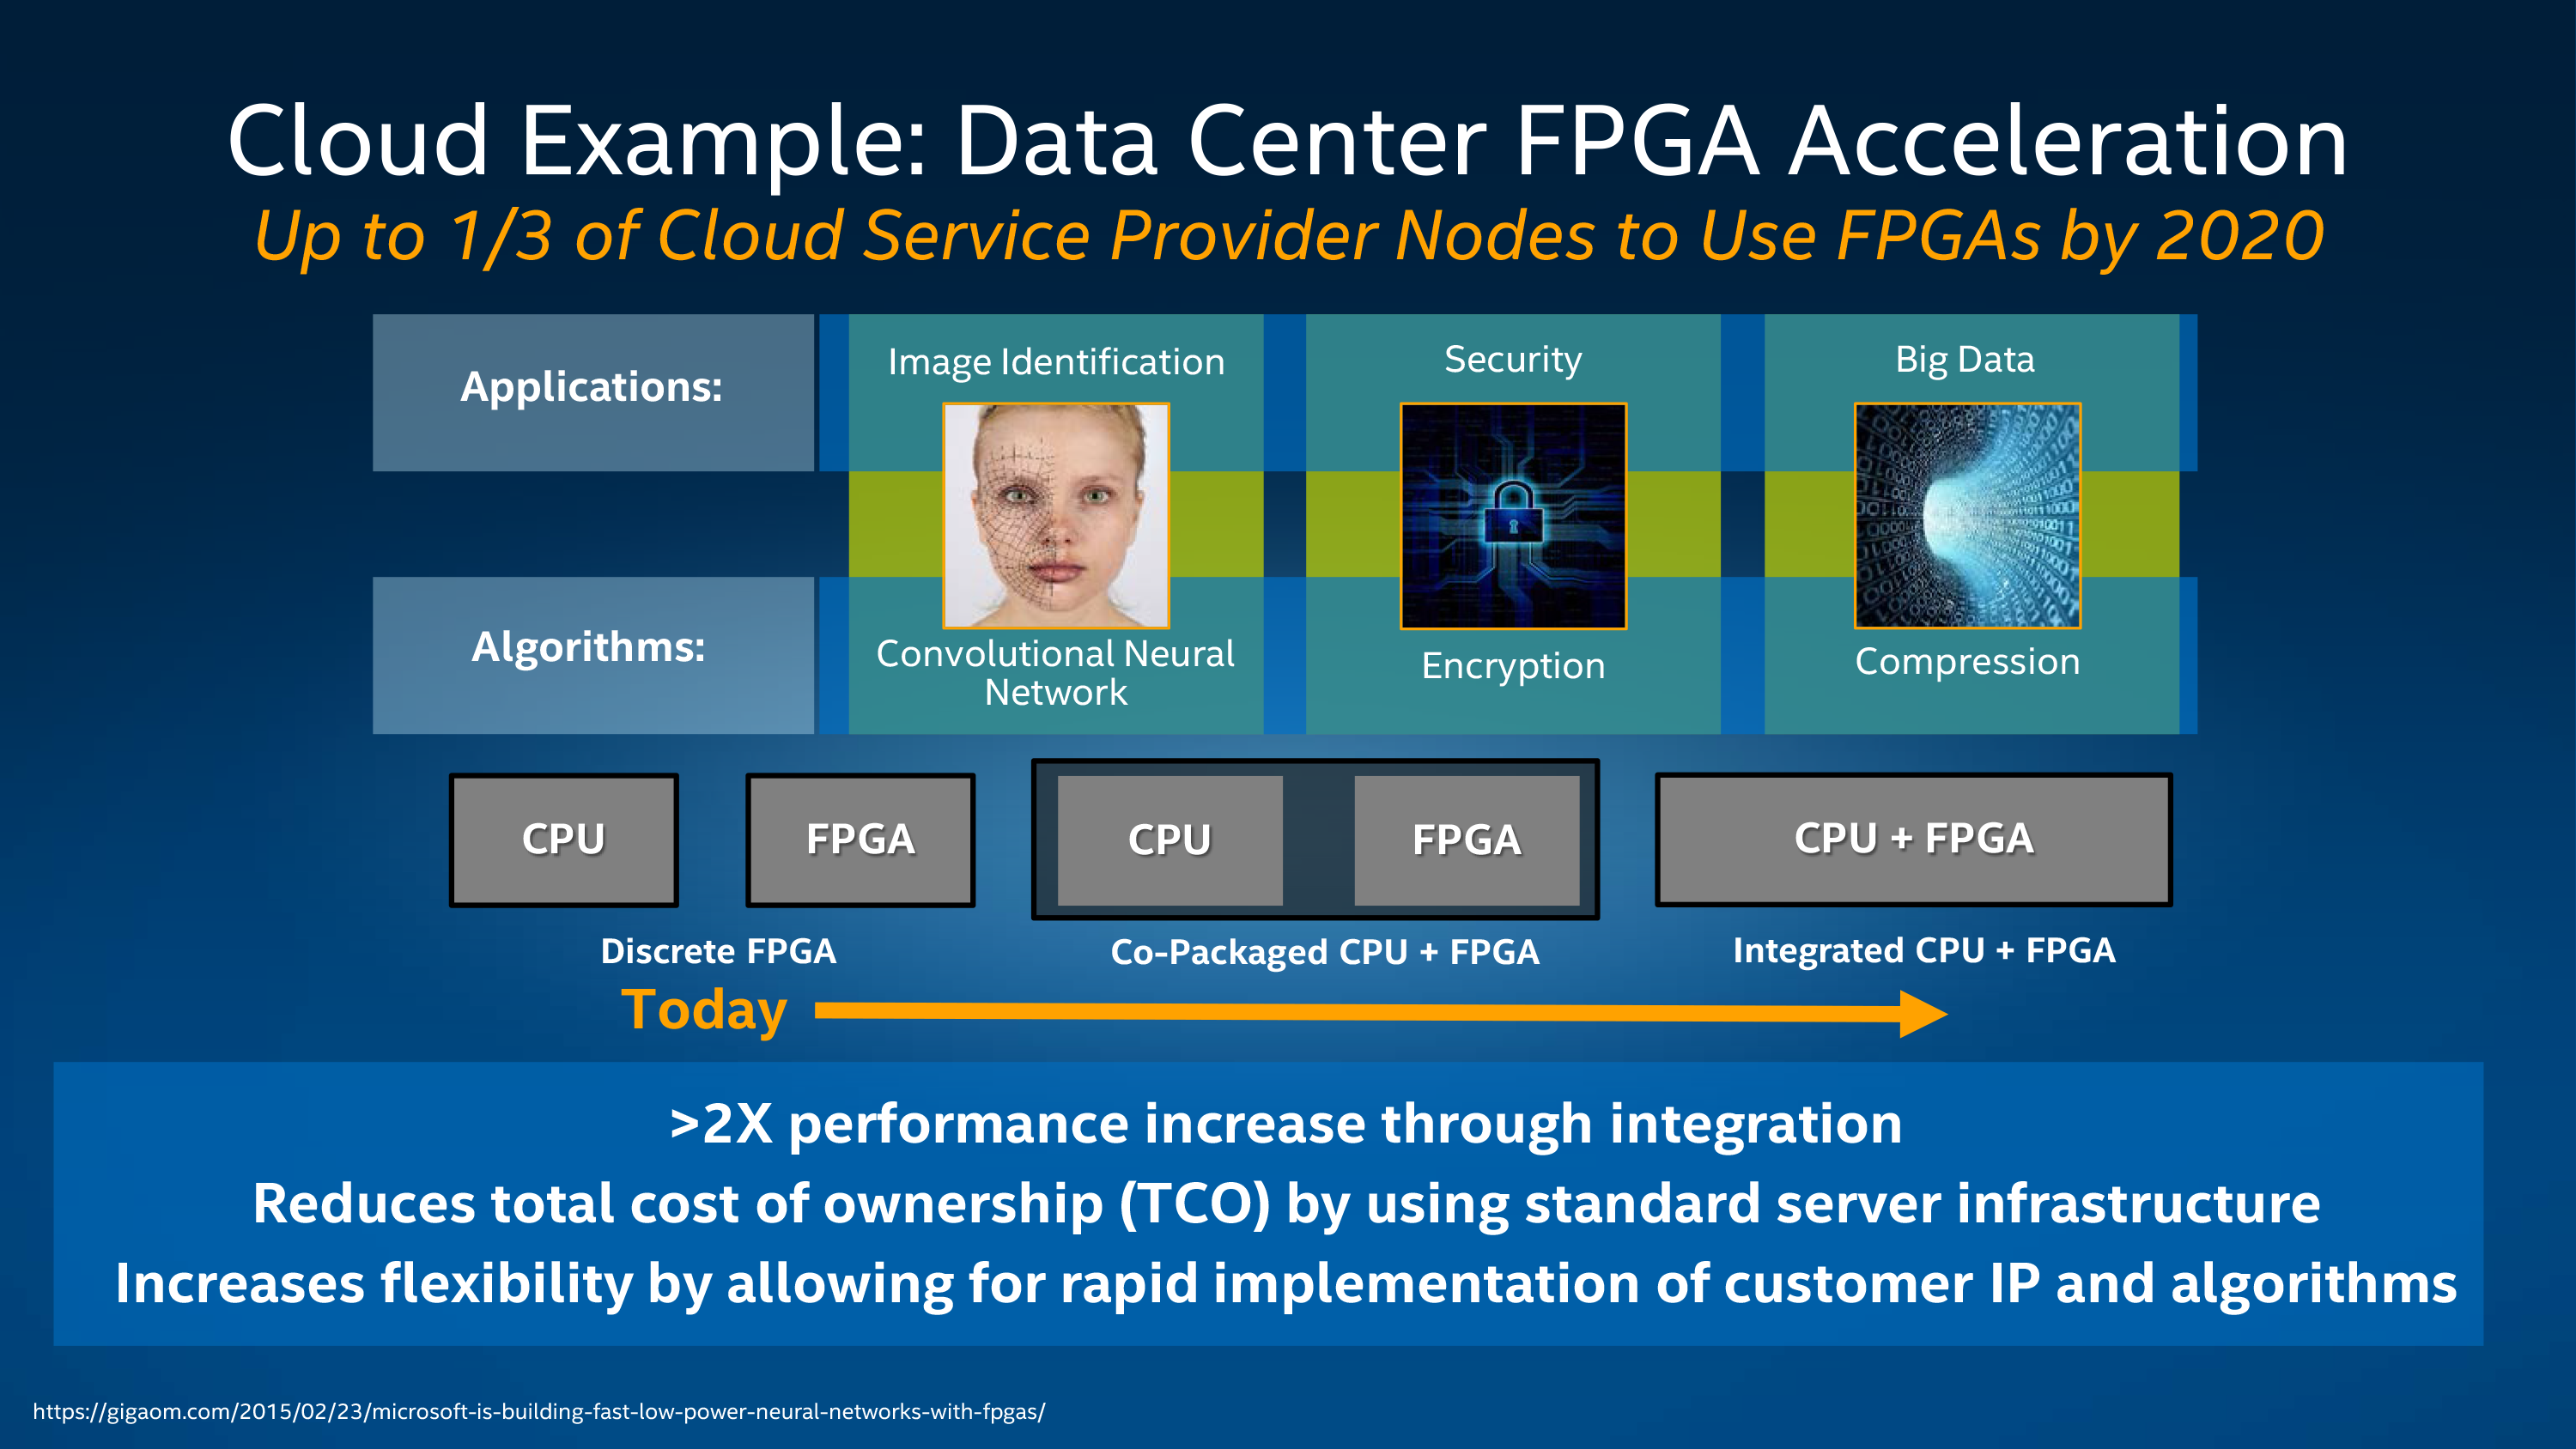
\includegraphics[width=\textwidth]{fpga2020}
    \end{center}

    \vfill

    \begin{center}
        \scriptsize{Fonte: anandtech.com/show/9321/intel-to-acquire-fpgaspecialist-altera-for-167-billion}
    \end{center}
\end{frame}

\subsection{Arquitetura de FPGAs: Lógica Programável}

\begin{frame}
    \frametitle{Arquitetura de Memória: Lógica Programável}
    \begin{center}
        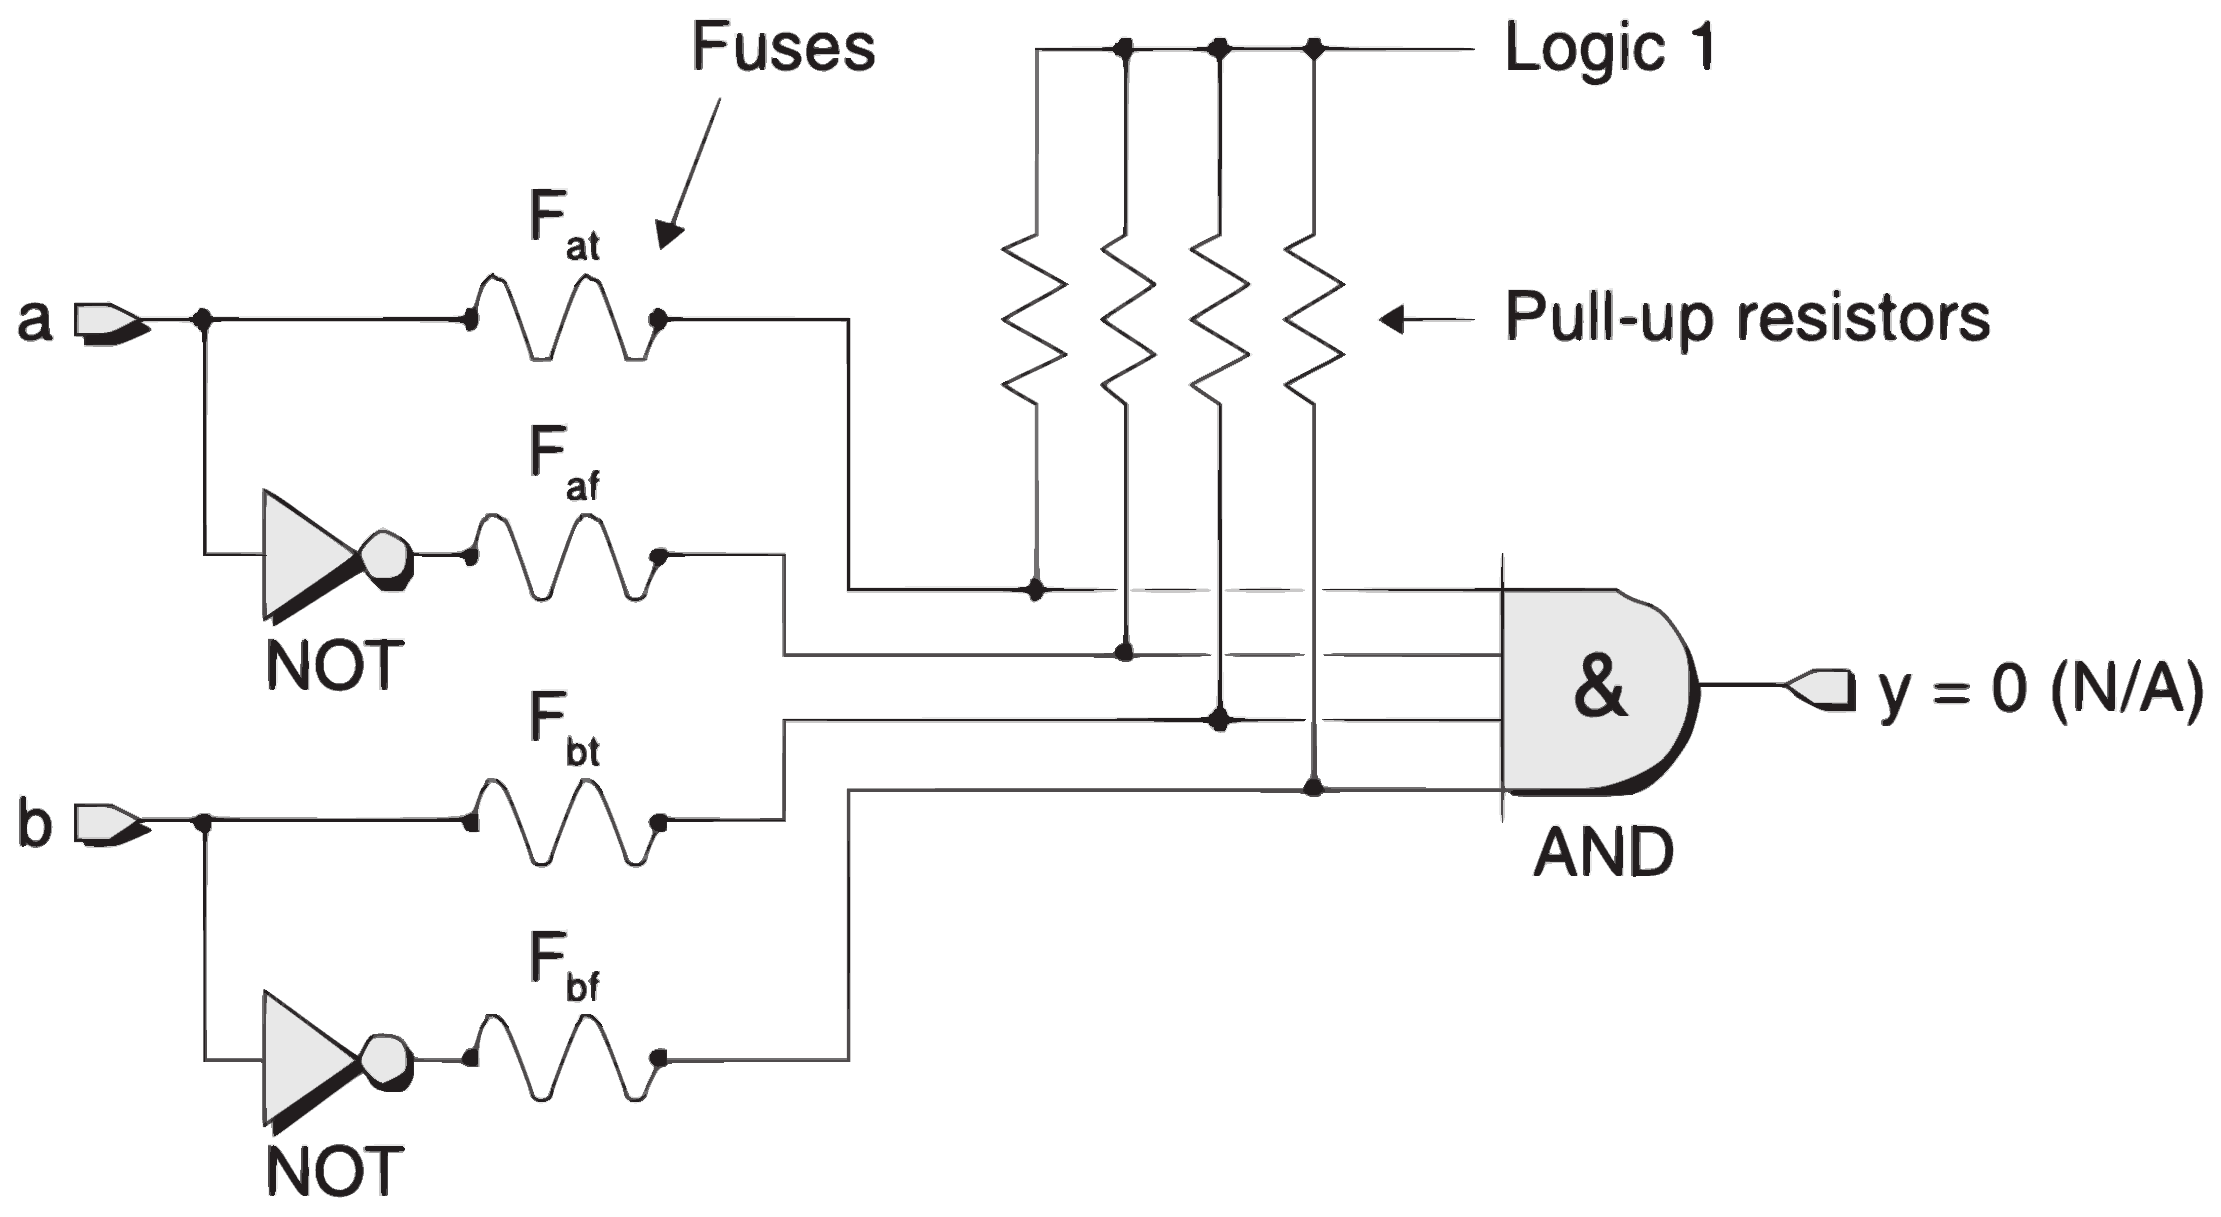
\includegraphics[width=.75\textwidth]{fusible-link}
    \end{center}

    \vfill

    \begin{center}
        \scriptsize{Fonte: Maxfield, Clive. The design warrior's guide to FPGAs: devices, tools and flows. Elsevier, 2004.}
    \end{center}
\end{frame}

\begin{frame}
    \frametitle{Arquitetura de Memória: Lógica Programável}
    \begin{center}
        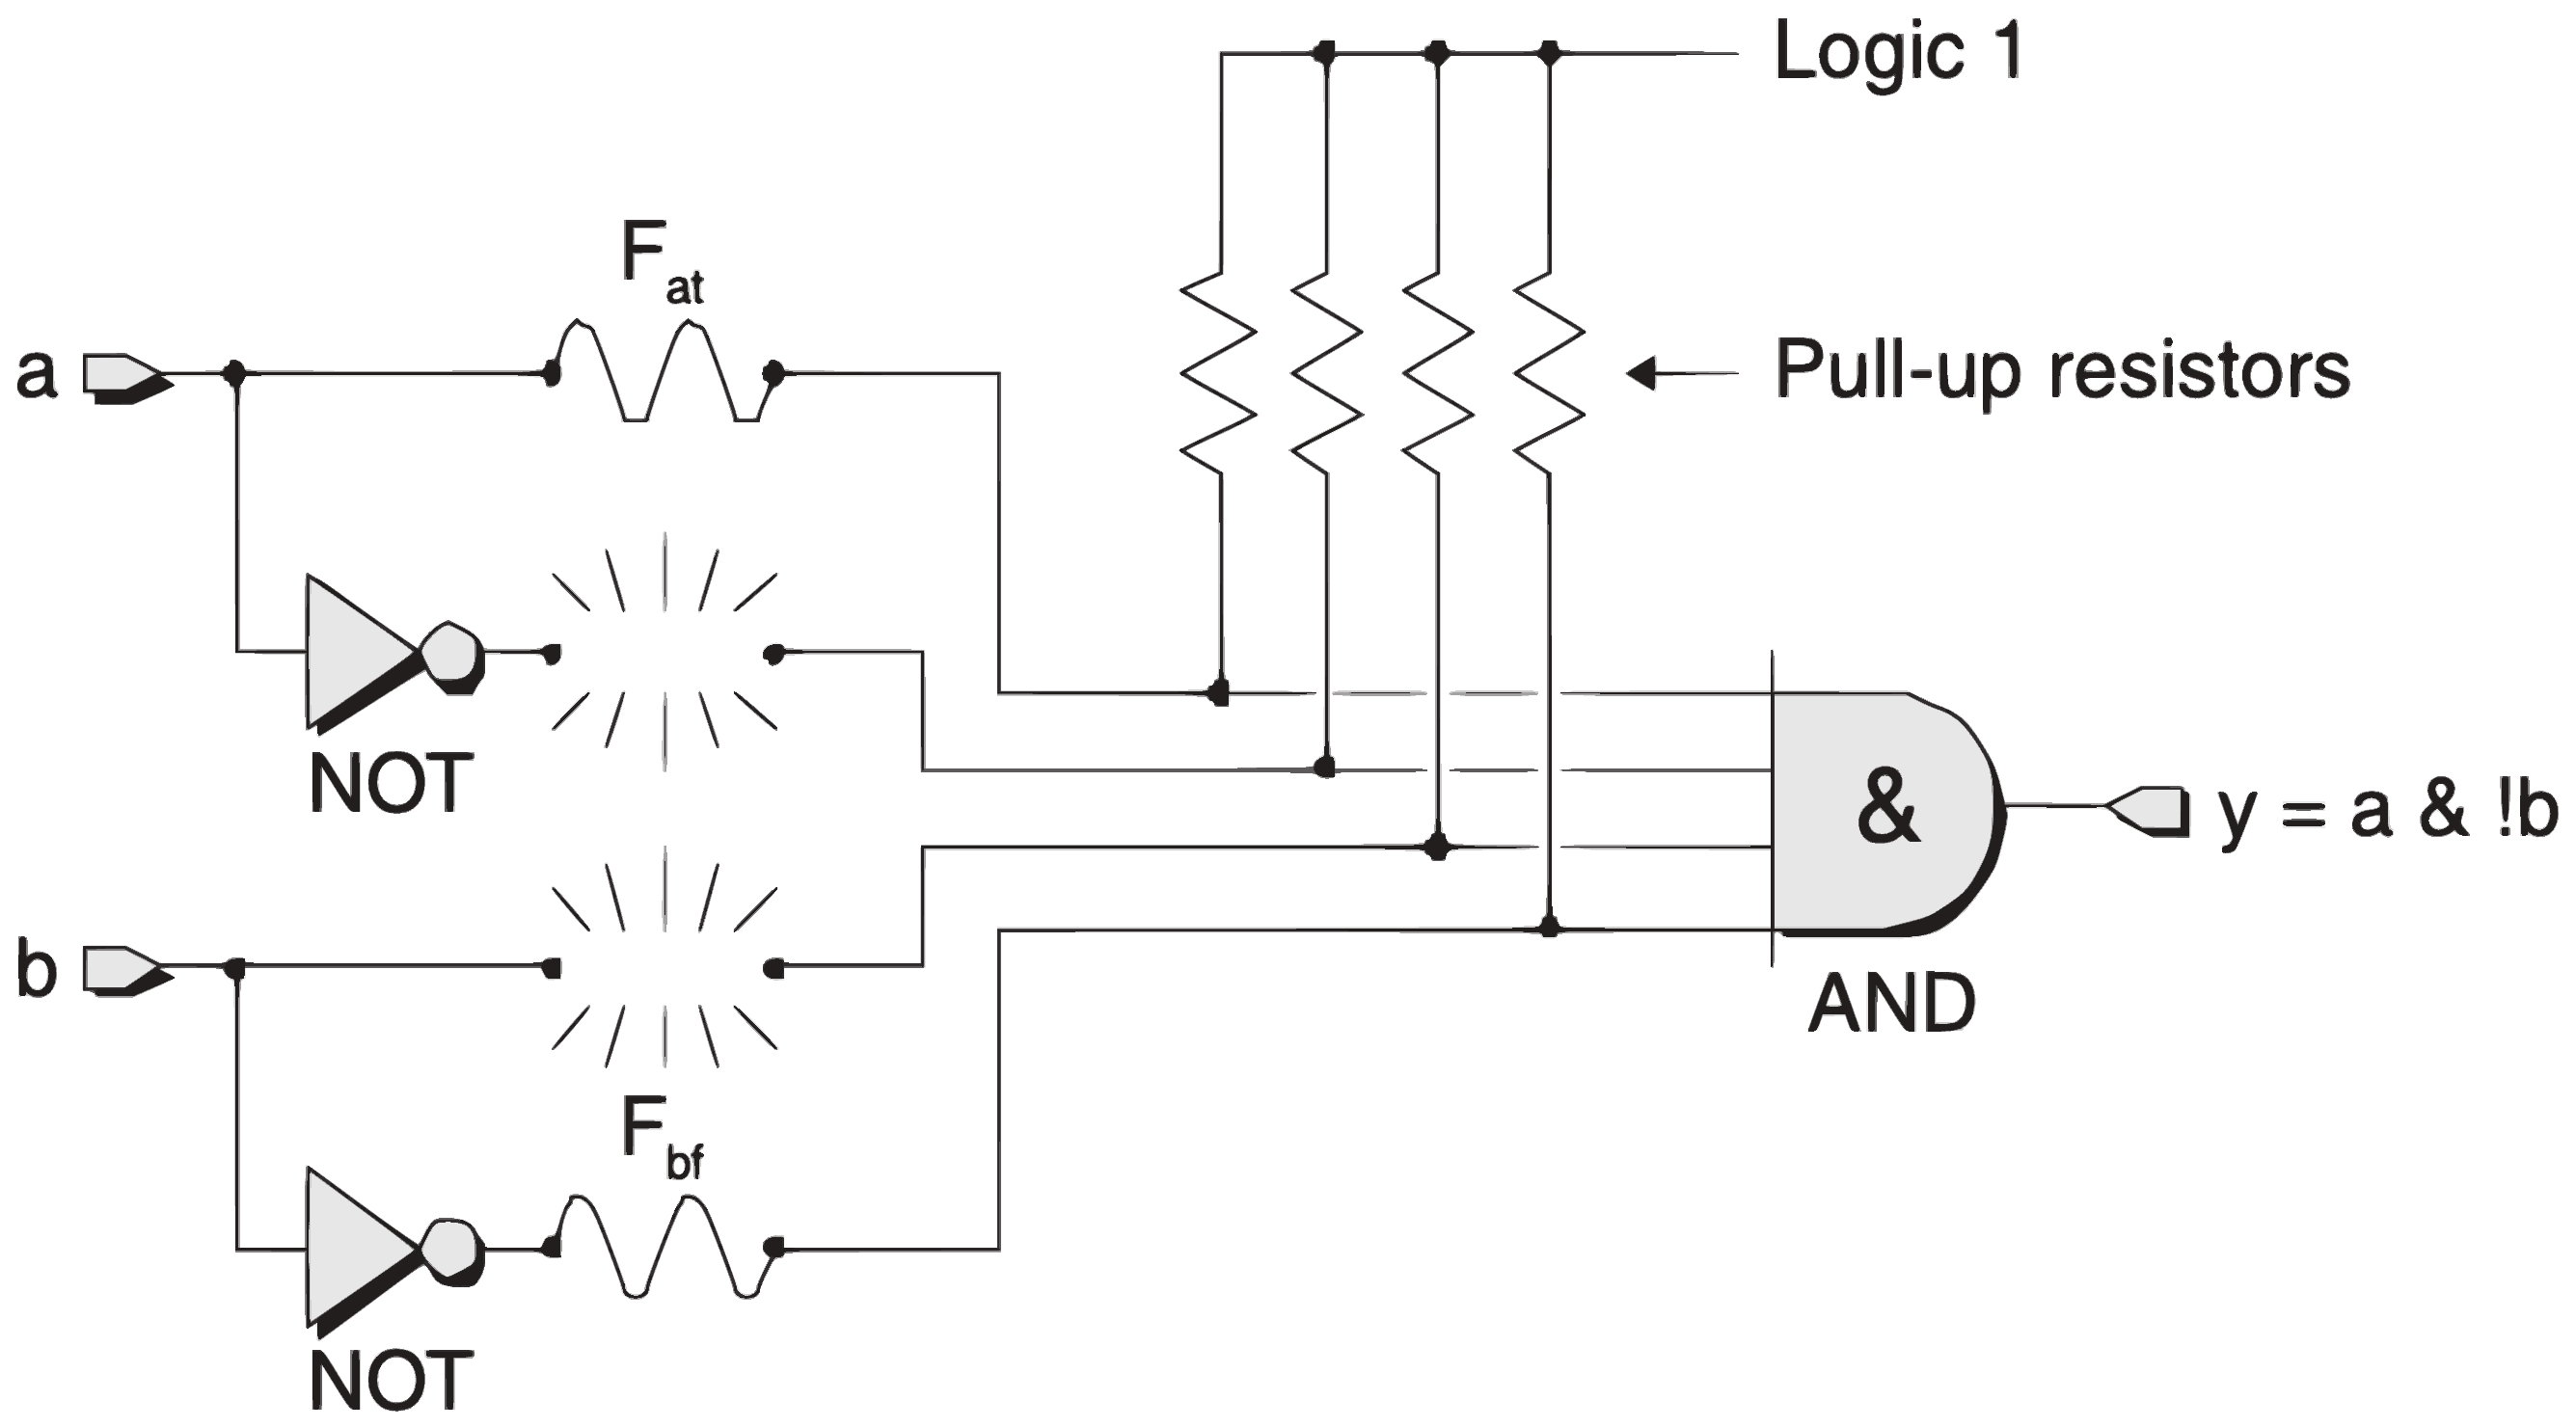
\includegraphics[width=.75\textwidth]{fusible-programmed}
    \end{center}

    \vfill

    \begin{center}
        \scriptsize{Fonte: Maxfield, Clive. The design warrior's guide to FPGAs: devices, tools and flows. Elsevier, 2004.}
    \end{center}
\end{frame}

\begin{frame}
    \frametitle{Arquitetura de Memória: EPROM}
    \begin{center}
        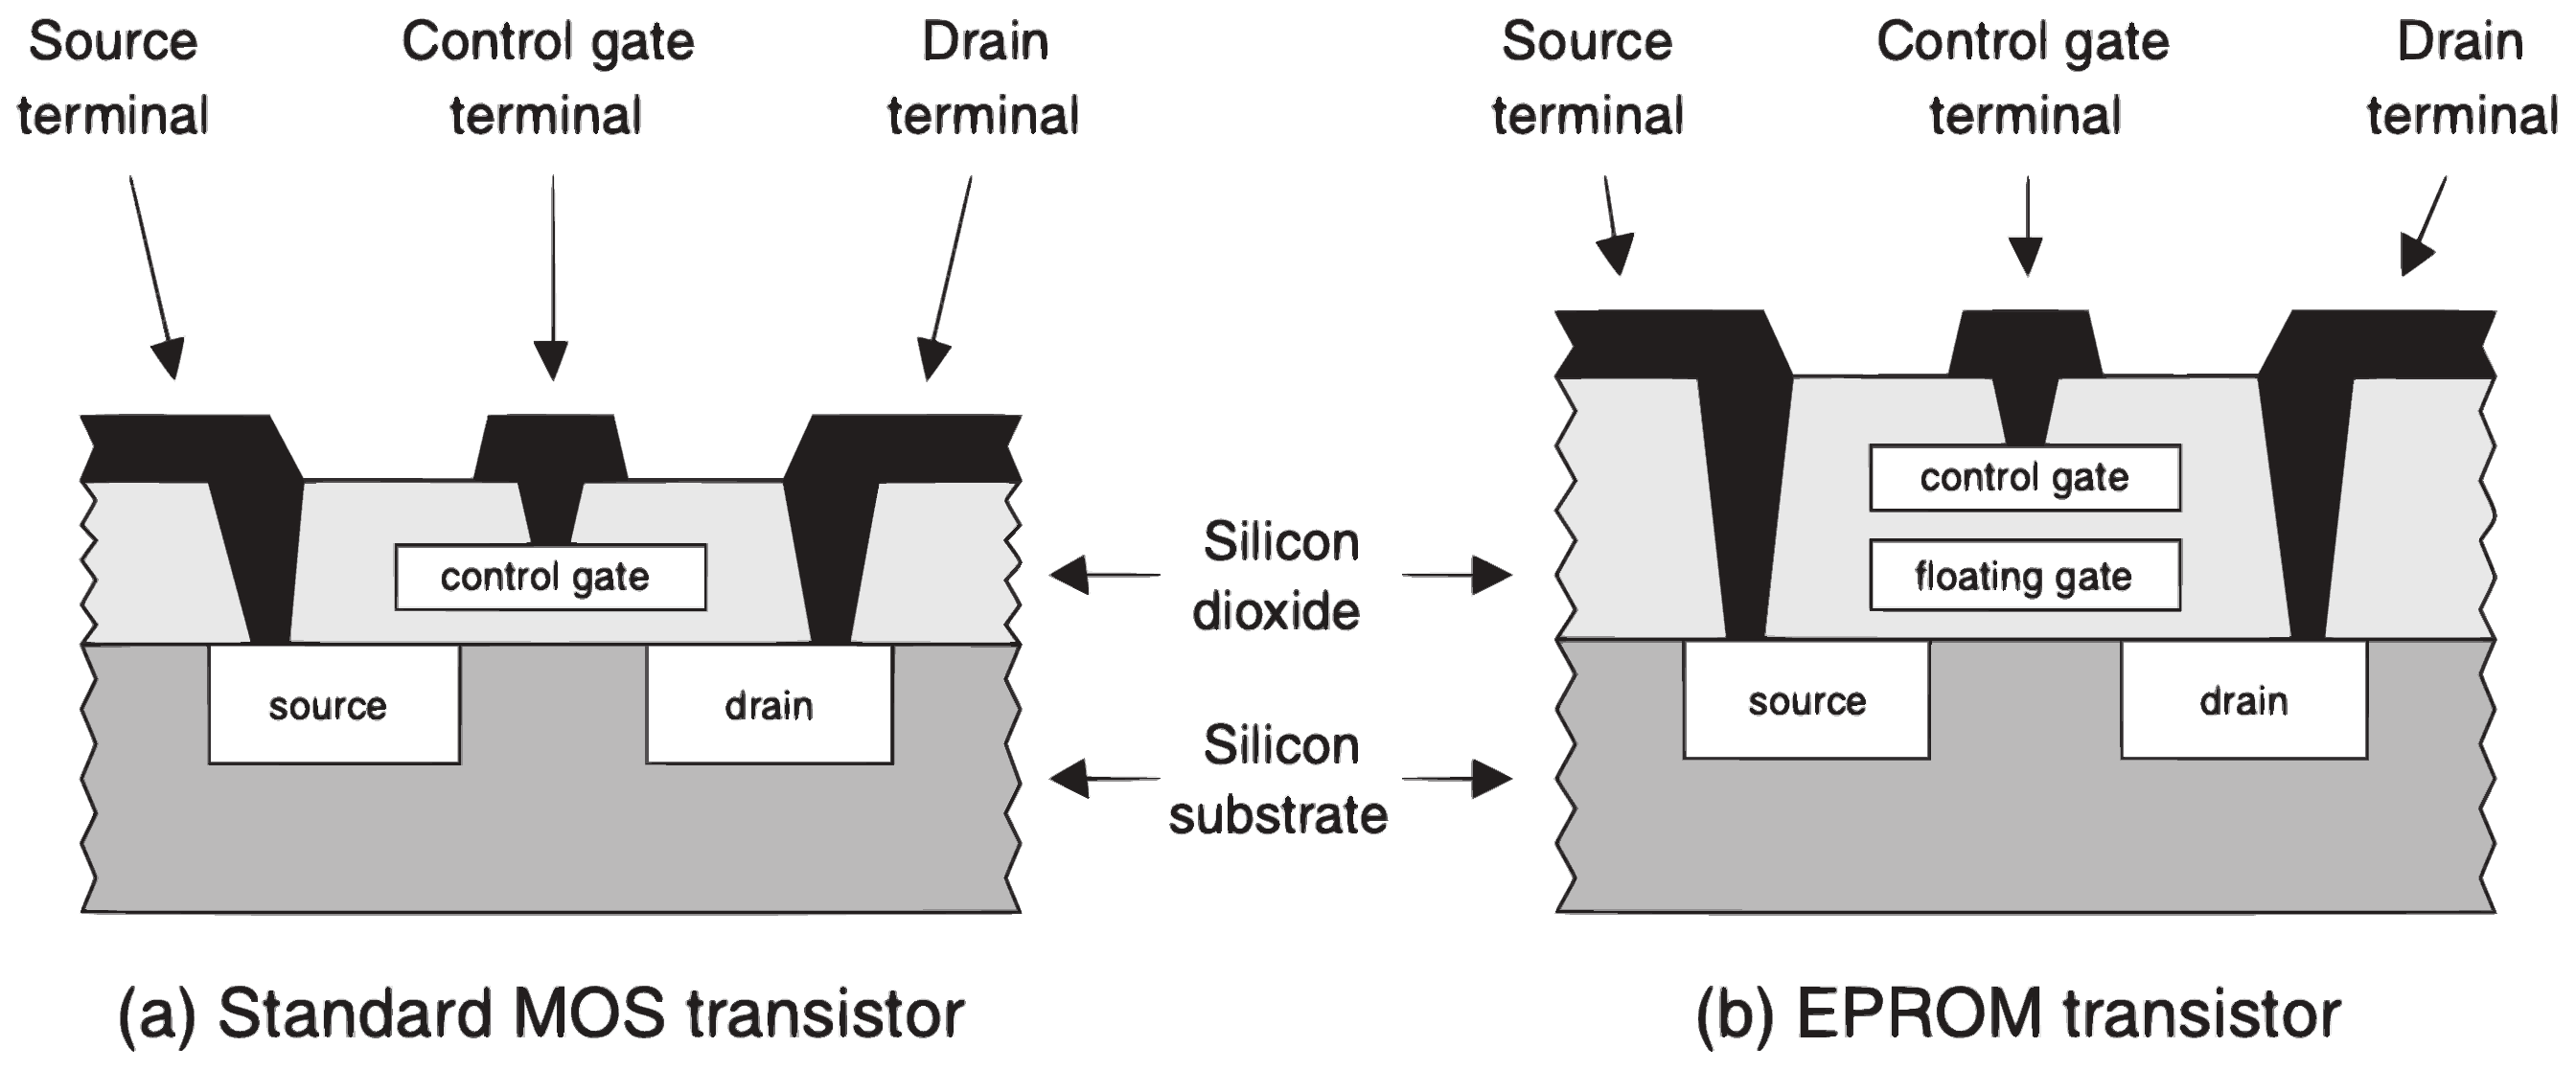
\includegraphics[width=.75\textwidth]{eprom-transistor}
    \end{center}

    \vfill

    \begin{center}
        \scriptsize{Fonte: Maxfield, Clive. The design warrior's guide to FPGAs: devices, tools and flows. Elsevier, 2004.}
    \end{center}
\end{frame}

\begin{frame}
    \frametitle{Arquitetura de FPGAs}
    Arquitetura de Memória:
    \begin{itemize}
        \item Lógica Programável: Static Random Access Memory (\alert{SRAM})
        \item Memória: Synchronous Dynamic Random Access Memory (\alert{SDRAM})
    \end{itemize}

    \pause
    \alert{2D Gate Arrays}:

    \begin{itemize}
        \item Elementos Lógicos: Portas Lógicas, Transistores (\alert{LEs})
        \item Conexões entre LEs: \alert{Interconnect}
        \item Tabelas de Verdade: \textit{Lookup Tables} (\alert{LUTs})
    \end{itemize}
\end{frame}

\begin{frame}[fragile]
    \frametitle{FPGAs: Visão Simplificada de Alto Nível}
    \begin{center}
        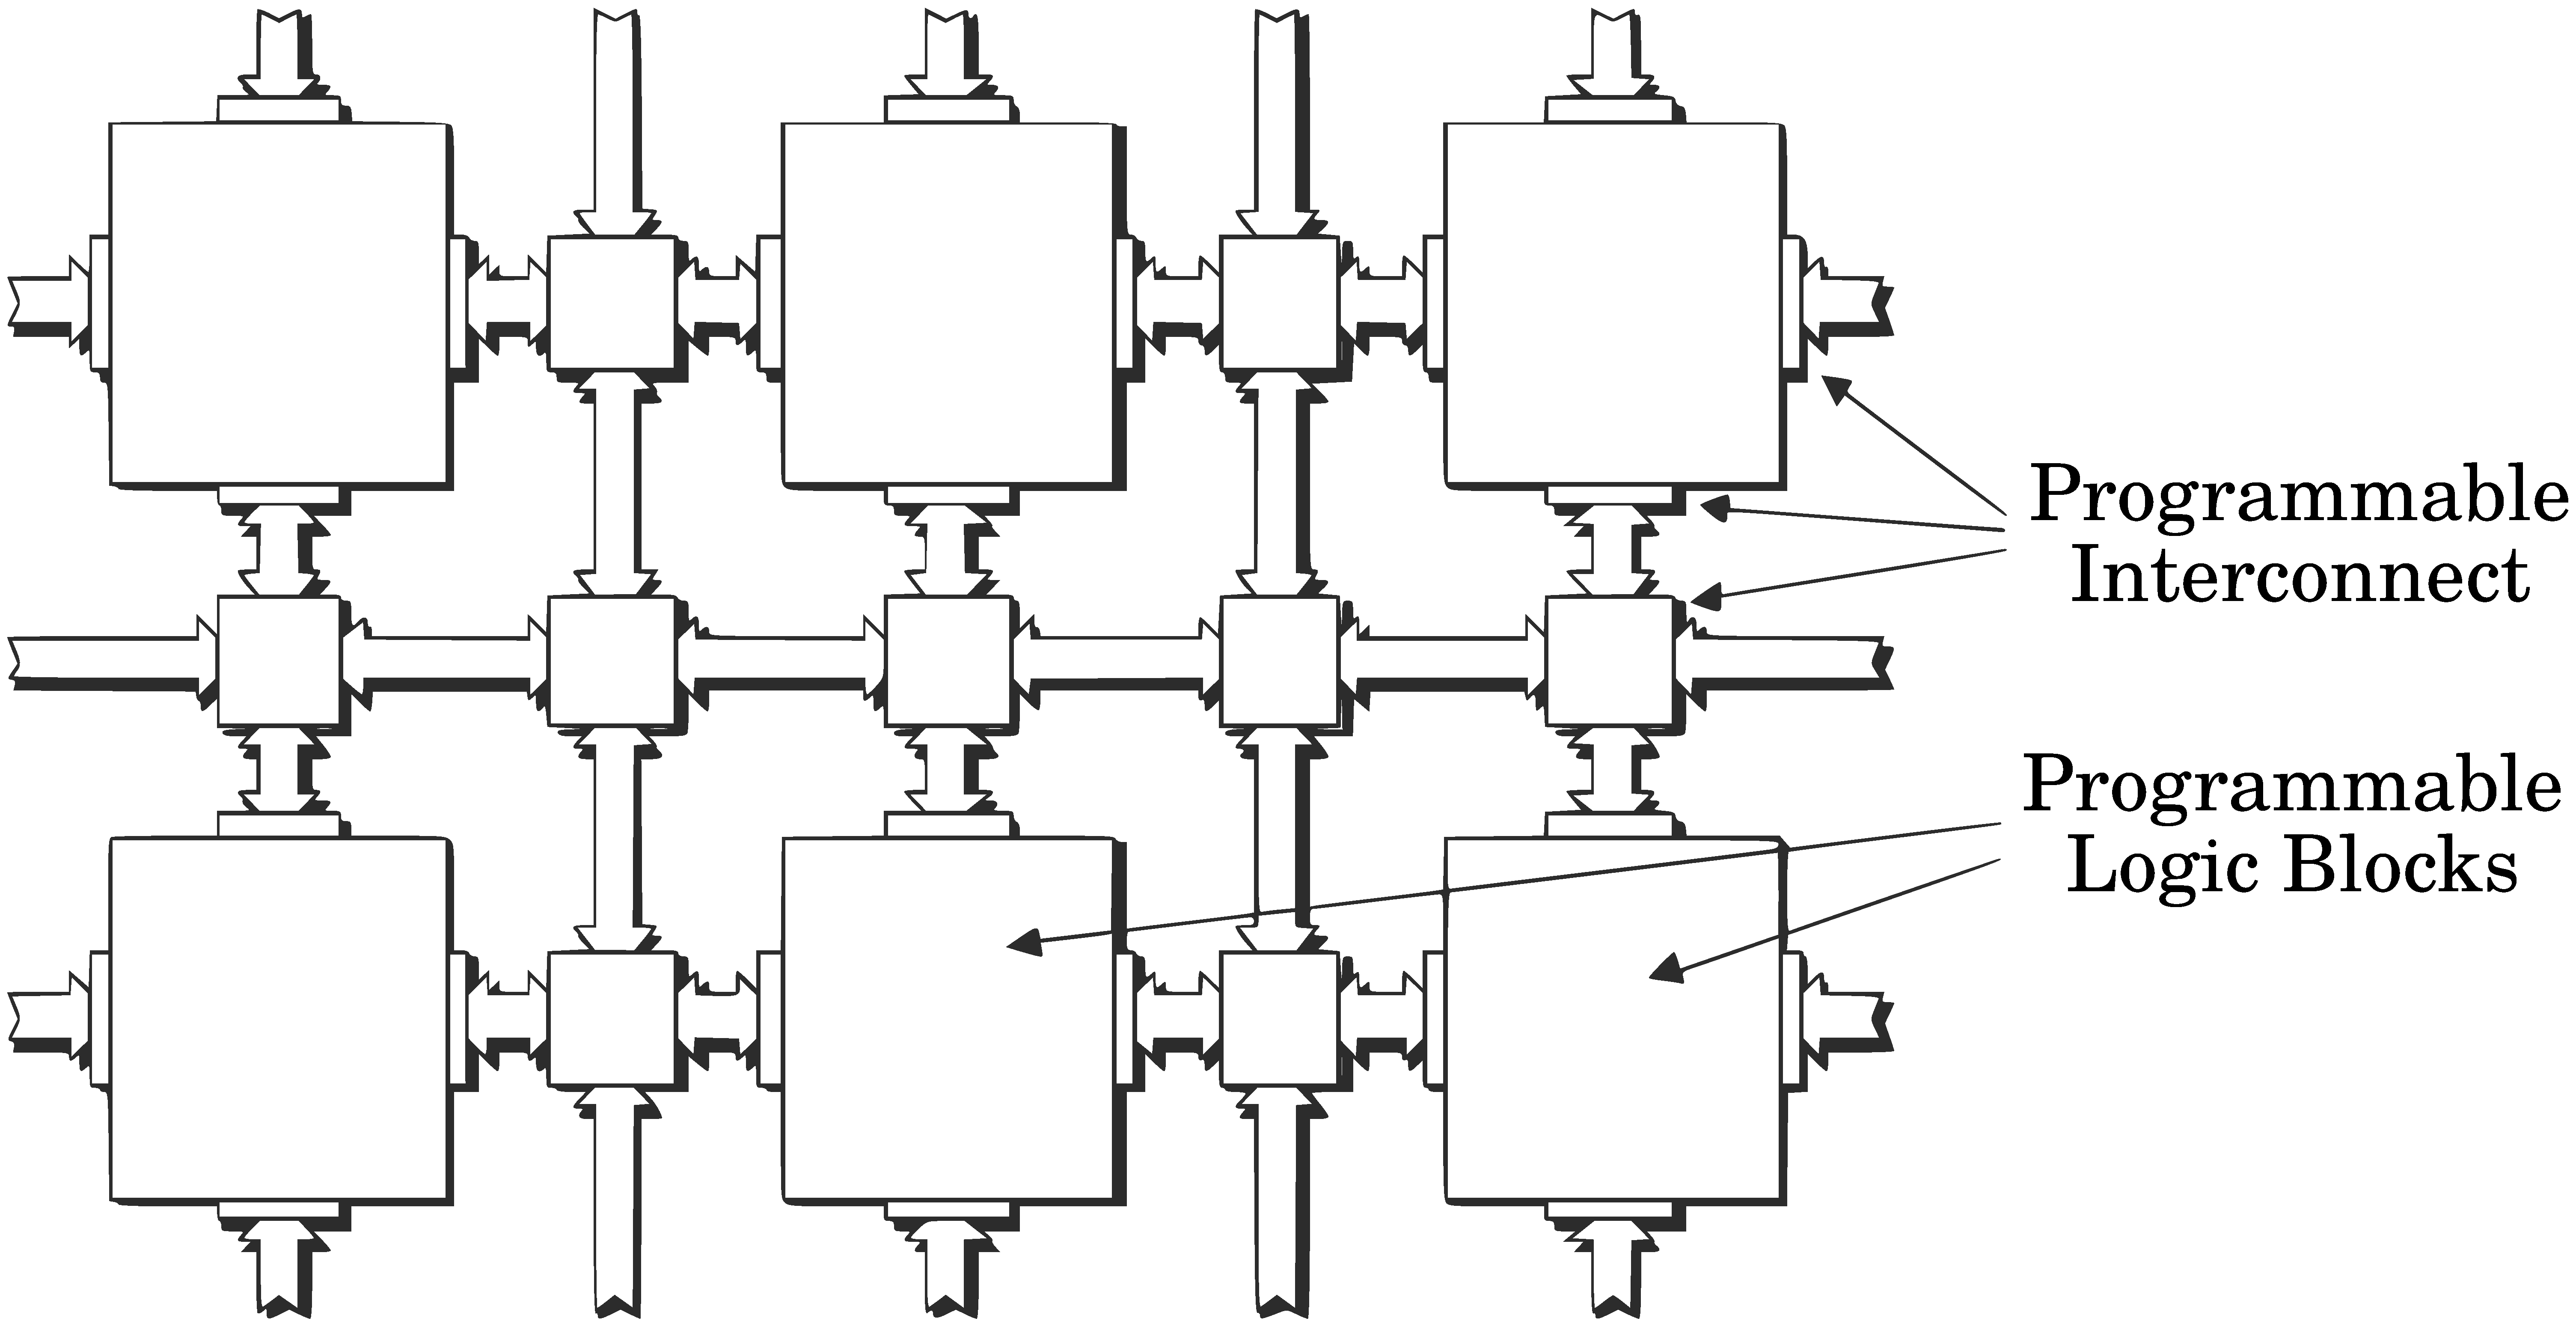
\includegraphics[width=\textwidth]{FPGA_simple}
    \end{center}

    \vfill

    \begin{center}
        \scriptsize{Fonte: Maxfield, Clive. The design warrior's guide to FPGAs: devices, tools and flows. Elsevier, 2004.}
    \end{center}
\end{frame}

\begin{frame}
    \frametitle{FPGAs: Visão Simplificada de Baixo Nível}
    \begin{center}
        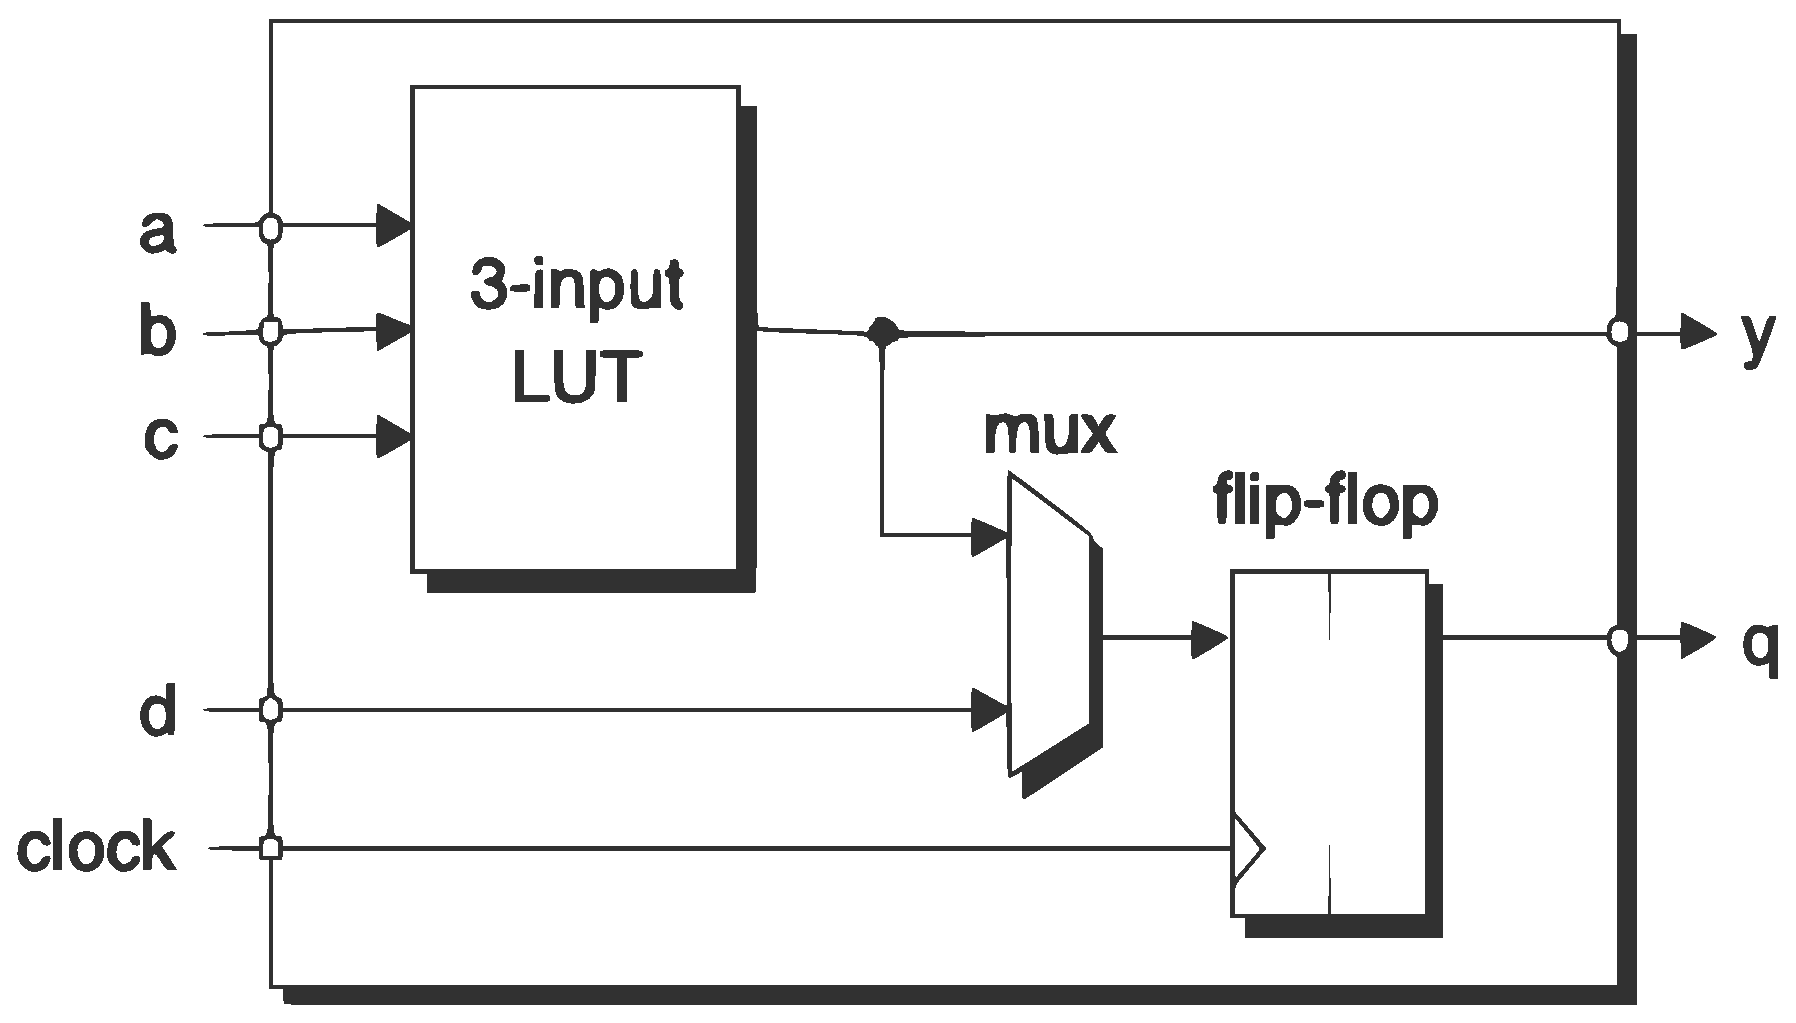
\includegraphics[width=.75\textwidth]{logic-block}
    \end{center}

    \vfill

    \begin{center}
        \scriptsize{Fonte: Maxfield, Clive. The design warrior's guide to FPGAs: devices, tools and flows. Elsevier, 2004.}
    \end{center}
\end{frame}

\begin{frame}
    \frametitle{FPGAs: Visão Simplificada de Baixo Nível}
    \begin{center}
        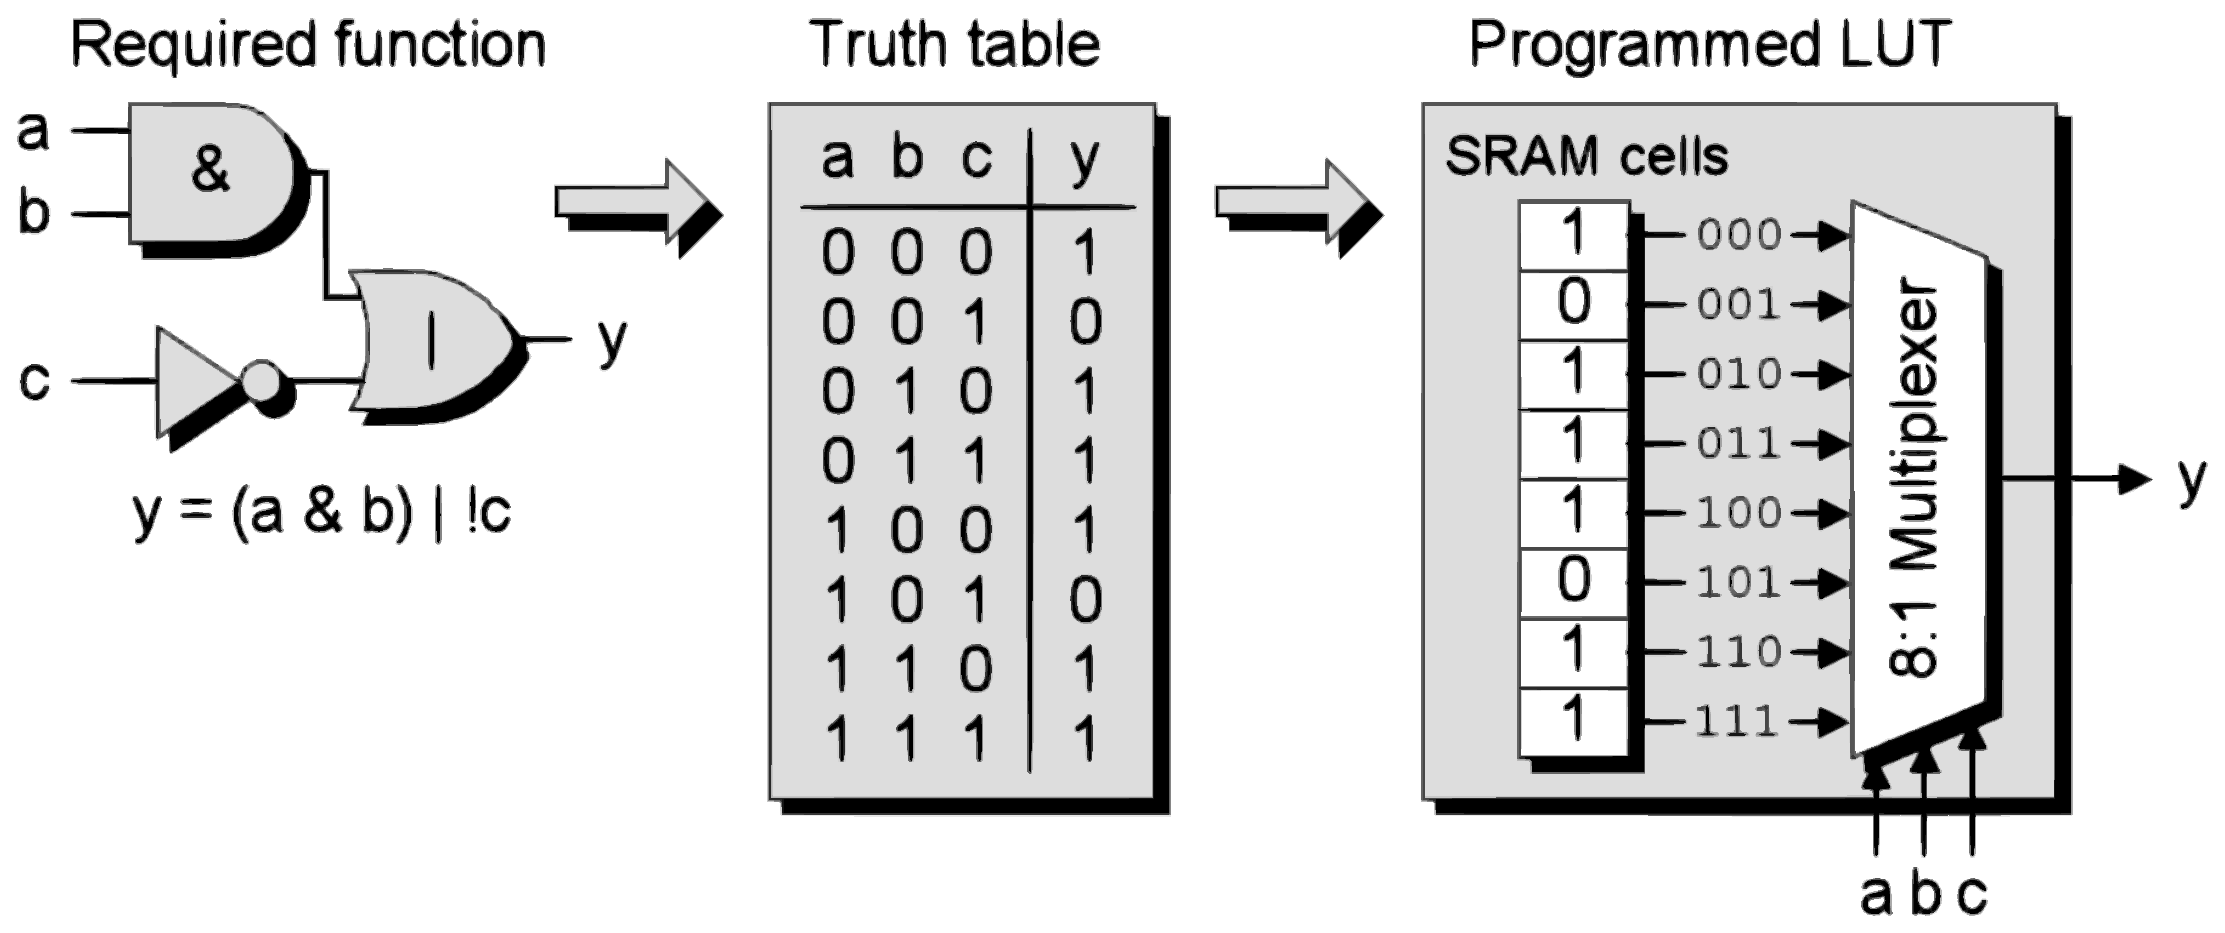
\includegraphics[width=.76\textwidth]{lut}
    \end{center}

    \vfill

    \begin{center}
        \scriptsize{Fonte: Maxfield, Clive. The design warrior's guide to FPGAs: devices, tools and flows. Elsevier, 2004.}
    \end{center}
\end{frame}

\begin{frame}
    \frametitle{FPGAs Hoje}
    Arquitetura de FPGAs contemporânea:
    \begin{itemize}
        \item Associada a uma \alert{CPU}
        \item Static Random Access Memory (\alert{SRAM})
        \item Synchronous Dynamic Random Access Memory (\alert{SDRAM})
        \item \alert{I/O}
        \item Elementos Lógicos (Logic Elements, \alert{LEs})
        \item Interconexões
    \end{itemize}
\end{frame}

\begin{frame}
    \frametitle{FPGAs SoC: Cyclone V}
    \begin{center}
        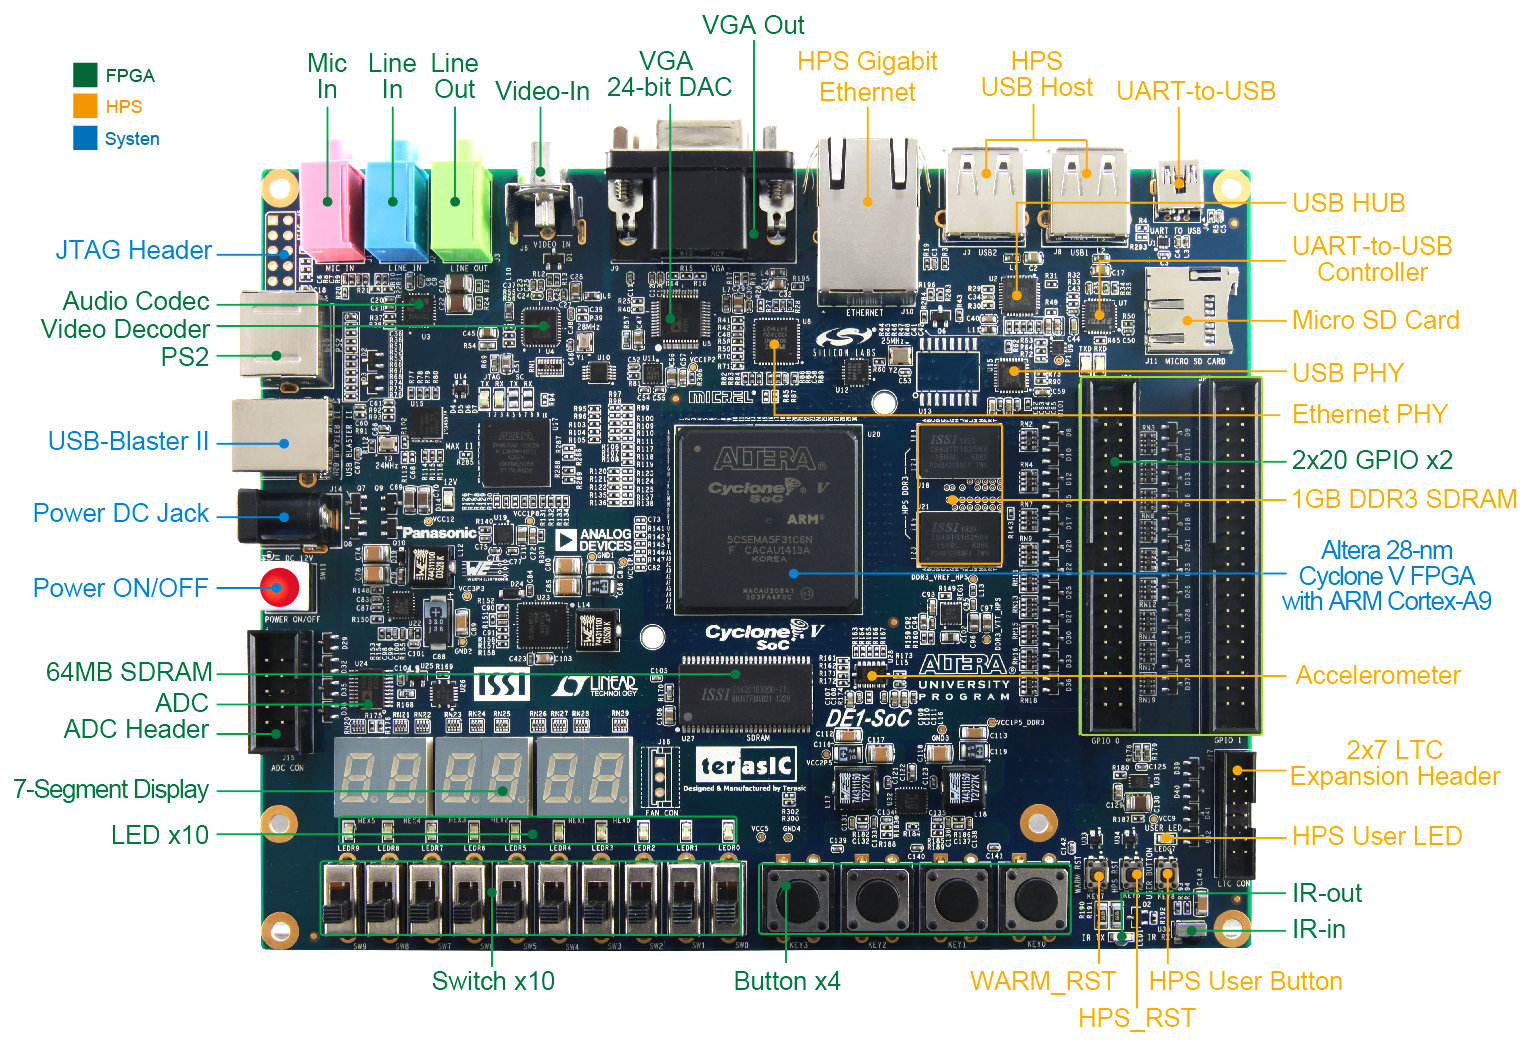
\includegraphics[width=\textwidth]{cycloneV}
    \end{center}
\end{frame}

\begin{frame}
    \frametitle{Programando FPGAs}
    Hardware Description Languages (\alert{HDL}):
    \begin{itemize}
        \item Definição de \textit{clock}
        \item Definição de circuitos e operações simples
        \item Hoje, muito já vem pré-definido
    \end{itemize}

    \pause

    High-Level Synthesis (\alert{HLS}):
    \begin{itemize}
        \item Gerar HDL a partir de \alert{código em C}
        \item \alert{OpenCL}
    \end{itemize}
\end{frame}

\begin{frame}
    \frametitle{FPGAs: Saiba Mais}
    Livros:

    \begin{itemize}
        \item Andrew Moore and Ron Wilson. FPGAs for Dummies. Intel/ Wiley, 2017
        \item Maxfield, Clive. The design warrior's guide to FPGAs: devices, tools and flows. Elsevier, 2004
        \item Vanderbauwhede, Wim, and Khaled Benkrid, eds. High-performance computing using FPGAs. New York: Springer, 2013 (Avançado)
    \end{itemize}
\end{frame}

\section{GPGPUs}

\subsection{História e Computação de Propósito Geral}

\begin{frame}
    \frametitle{GPUs: História e Computação de Propósito Geral}
    \begin{center}
        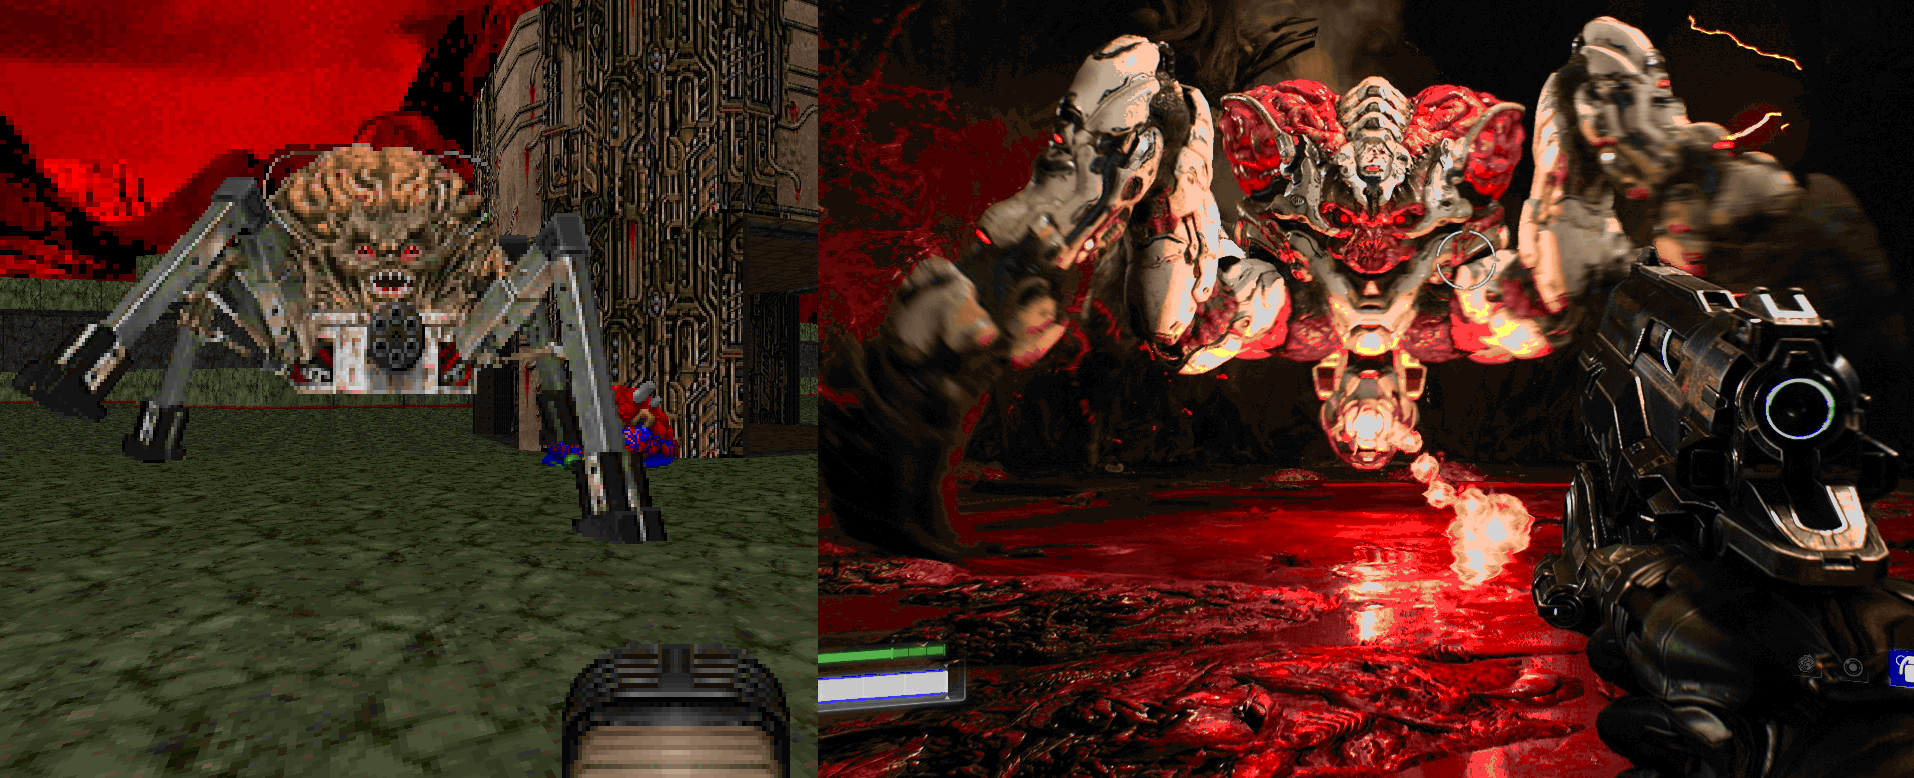
\includegraphics[width=\textwidth]{spiderdoom}
    \end{center}
\end{frame}

\frame{
\frametitle{Placas de Vídeo}
    \begin{minipage}{0.5\textwidth}
        \begin{itemize}
            \item 80's: Primeiro controlador de vídeo
            \item Evolução dos jogos 3D
            \item Aplicação de texturas, iluminação, sombras, $\dots$
            \item Animação, simulação computacional, design gráfico, física da luz, $\dots$
        \end{itemize}
    \end{minipage}\hfil
    \begin{minipage}{0.45\textwidth}
        \begin{figure}[htpb]
        \centering
        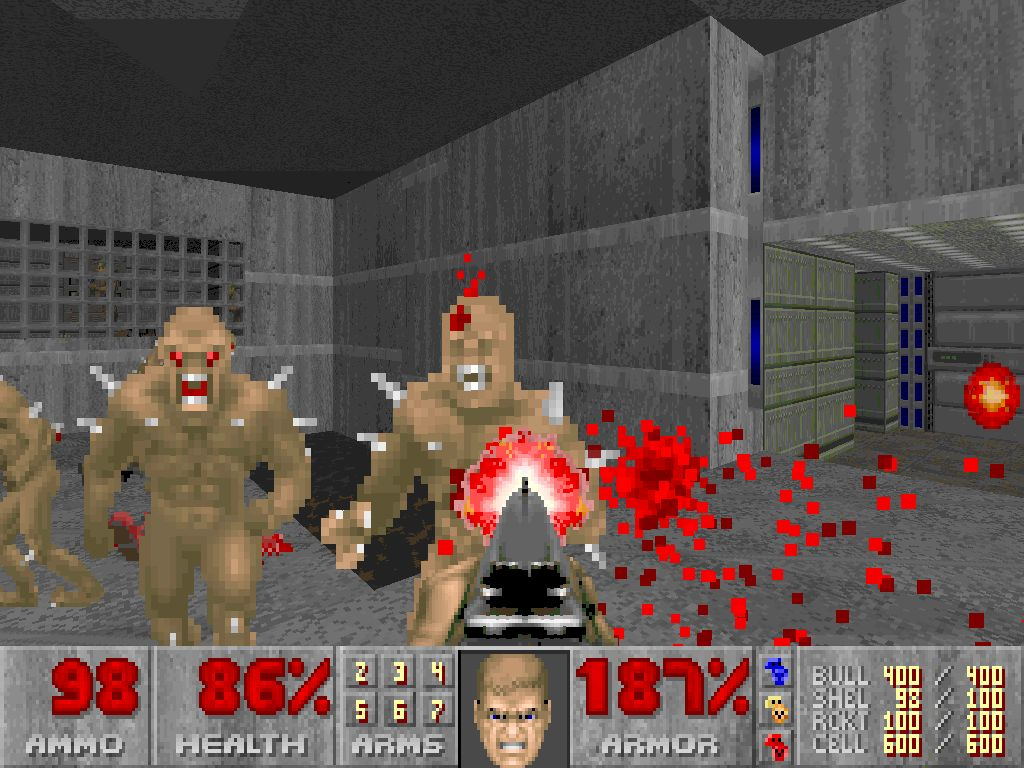
\includegraphics[scale=.175]{Doom-screenshots}\vspace{0.5cm}
        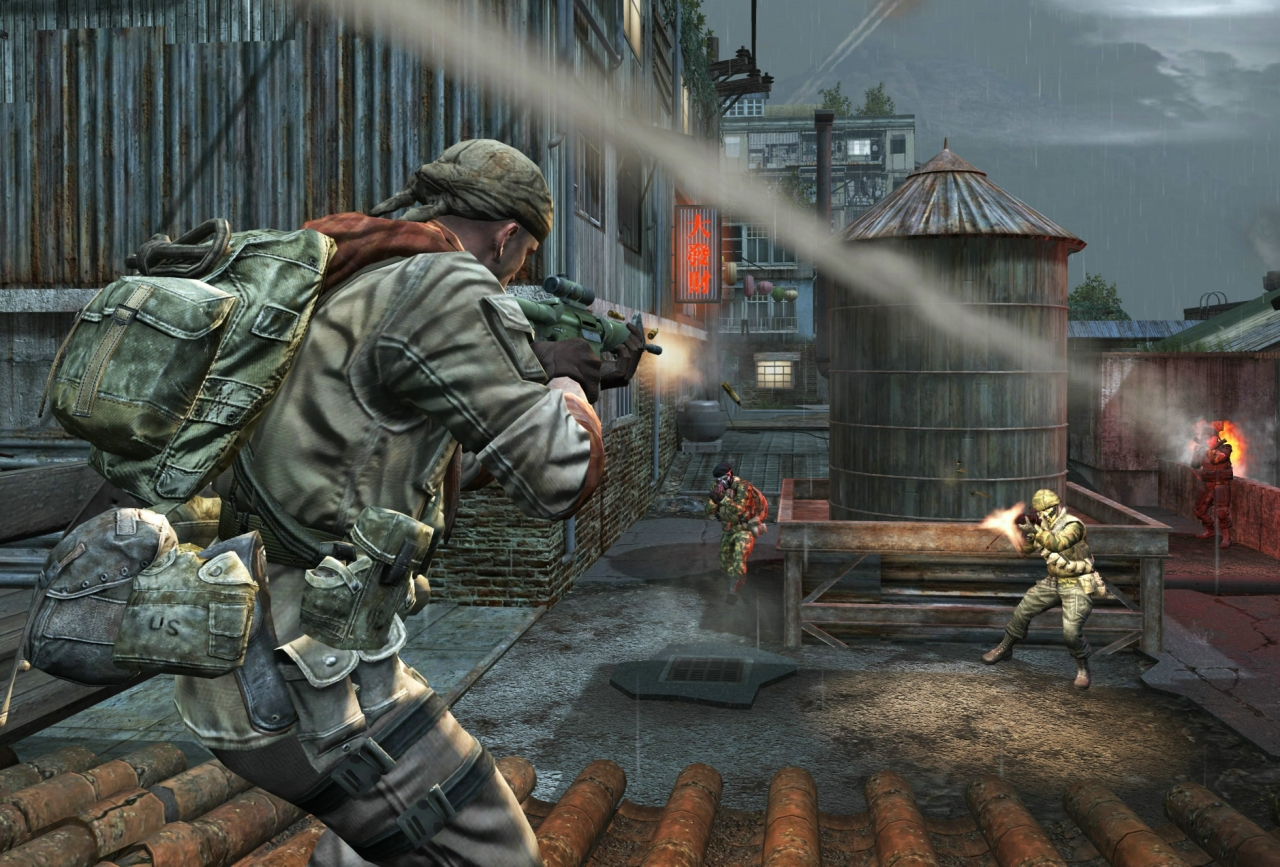
\includegraphics[scale=.135]{Call-of-Duty-Black-Ops}
        \label{fig:games3D}
        \end{figure}
    \end{minipage}
}

\frame{
    \frametitle{Unidades de Processamento Gráfico (GPUs)}
\small
\begin{minipage}{0.6\textwidth}
    \begin{itemize}
        \item O termo \alert{GPU} foi popularizado pela Nvidia em 1999, quando criou a GeForce 256
        \item Em 2002 foi lançada a primeira GPU de Propósito Geral (\alert{GPGPU})
        \item Os principais fabricantes de GPUs são a \alert{Nvidia} e a \alert{AMD}
        \item Em 2005 a Nvidia lançou \alert{CUDA}
        \item Inteligencia Artificial, Carros autônomos, Realidade Virtual, $\dots$
    \end{itemize}
\end{minipage}
\hfil
\begin{minipage}{0.35\textwidth}
    \begin{figure}[htpb]
        \centering
        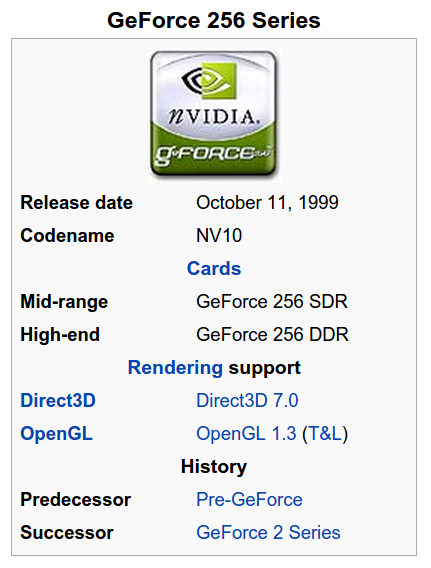
\includegraphics[scale=.3]{Geforce-256}
        \label{fig:GeForce-256}
    \end{figure}
\end{minipage}
}

\frame{
\frametitle{GPU vs. CPU}
\begin{block}{}
Hoje em dia, GPUs são capazes de fazer em paralelo mais operações computacionais que CPUs multi-core
\end{block}
\begin{figure}[h!]
\centering
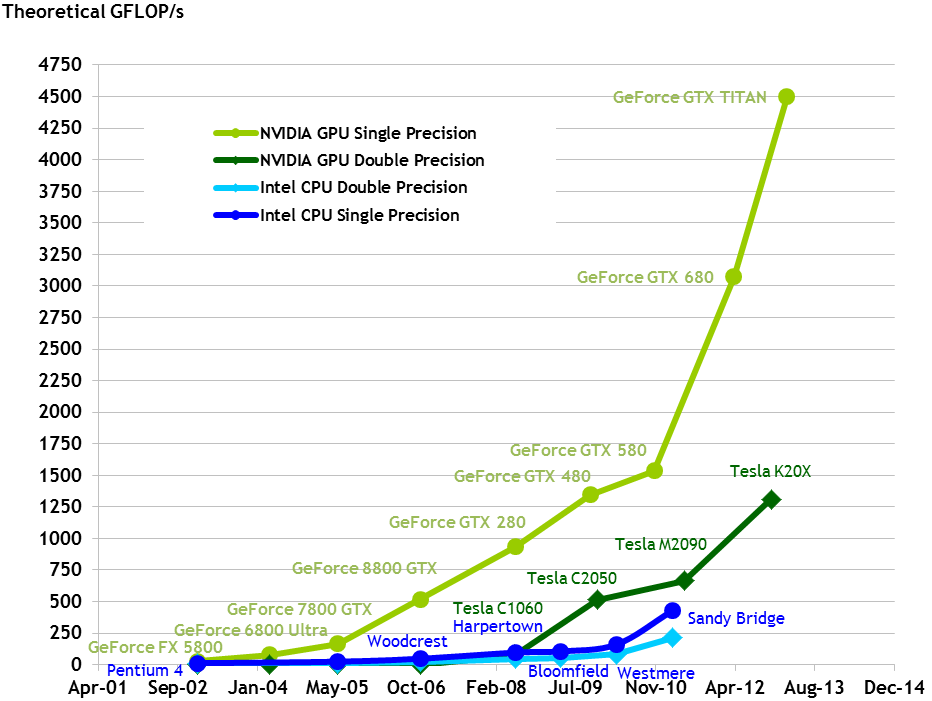
\includegraphics[scale=.175]{gflops}\hfill
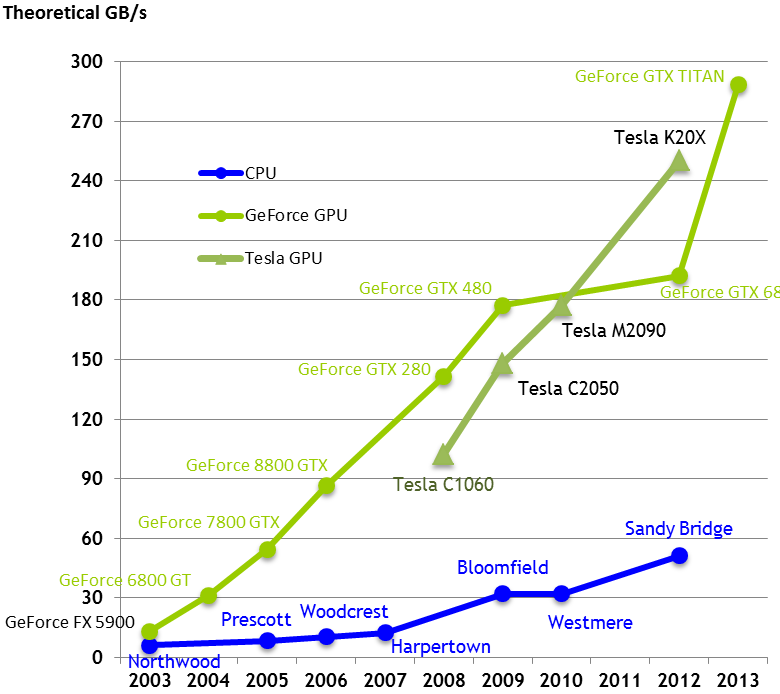
\includegraphics[scale=.175]{bandwidth}
\label{fig:gflops}
\end{figure}
}

\frame{
    \frametitle{GPU de Propósito Geral (GPGPU)}
O programa principal é executado na CPU (\alert{host}), que é responsável por
iniciar a execução na GPU (\alert{device}).

As GPUs têm sua própria herarquia de memória e os dados devem ser transferidos
através do barramento \alert{PCI Express}.

\centering
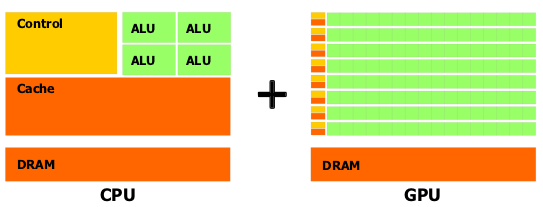
\includegraphics[scale=.75]{gpu-computing}
}

\frame{
\frametitle{Supercomputadores com Aceleradores de Hardware}
Supercomputadores na Top 500 com aceleradores e co-processadores:

\begin{figure}[htpb]
\centering
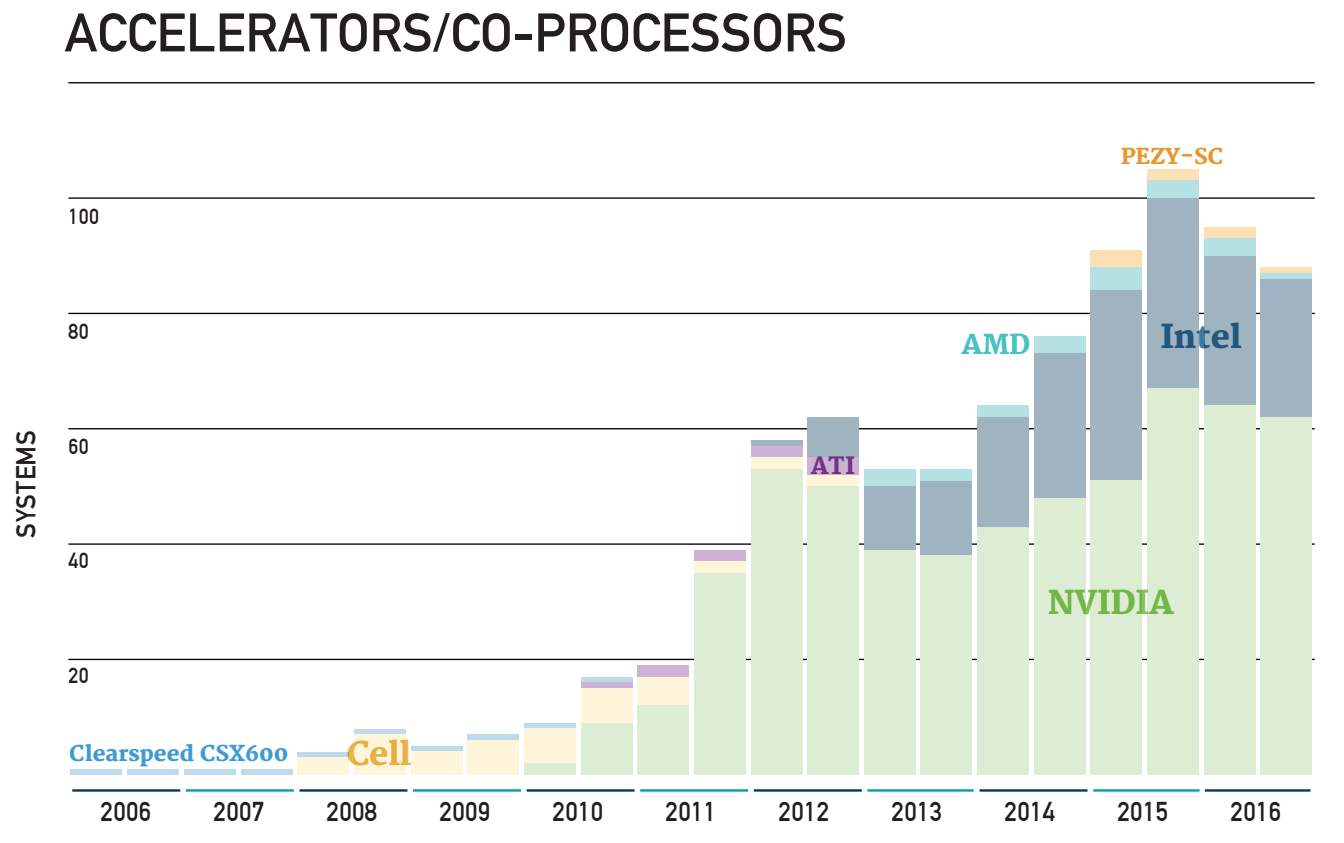
\includegraphics[scale=.225]{top-500-accelerators}
\label{fig:top500Acc}
\end{figure}
}

\frame{
\frametitle{Supercomputadores e Consumo de Energia}
\alert{Green 500}: Lista de supercomputadores mais eficientes em consumo de energia

\begin{figure}[htpb]
\centering
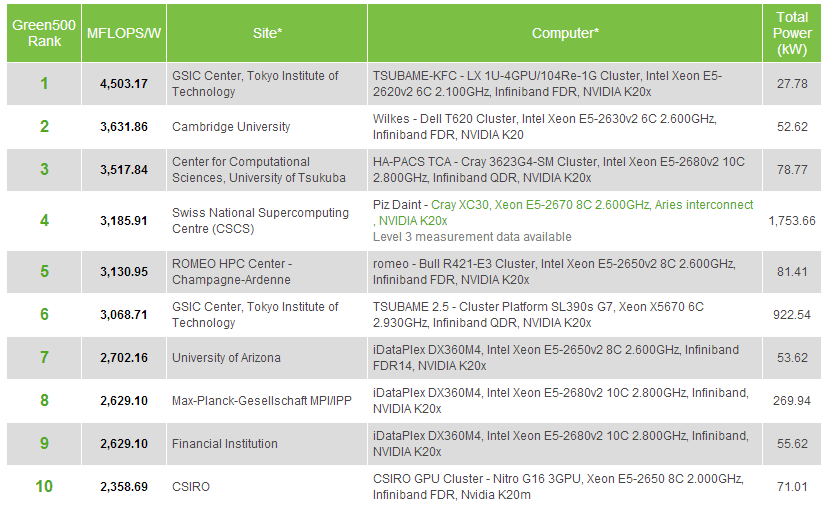
\includegraphics[scale=.36]{Green500Top10}
\label{fig:Grentop500}
\end{figure}
}

\subsection{GPGPUs Nvidia}

\begin{frame}
    \frametitle{GPGPUs Nvidia}
    \begin{center}
        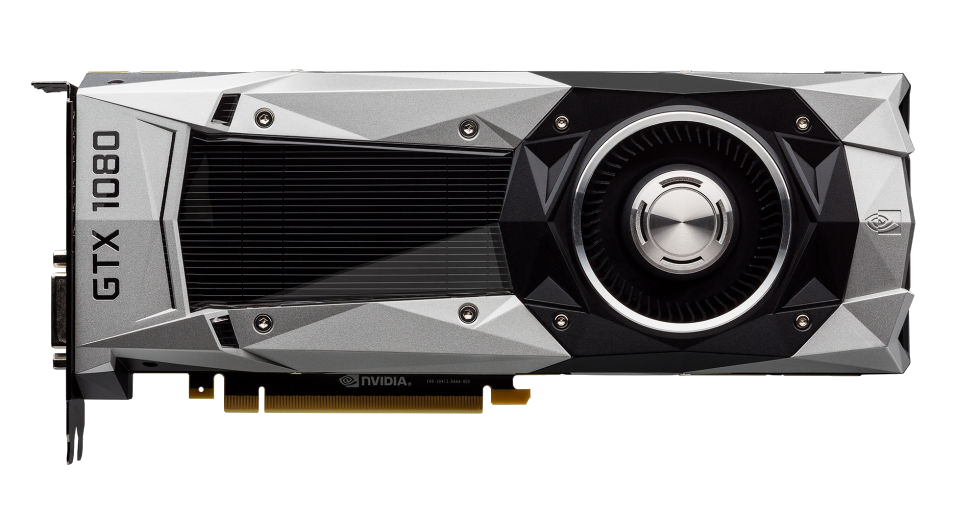
\includegraphics[width=\textwidth]{gtx1080}
    \end{center}
\end{frame}

\frame{
\frametitle{Roadmap para Arquiteturas de GPUs NVIDIA}
A próxima arquitetura será a Volta, com 12-10 nm FinFET.
\begin{figure}[htpb]
 \centering
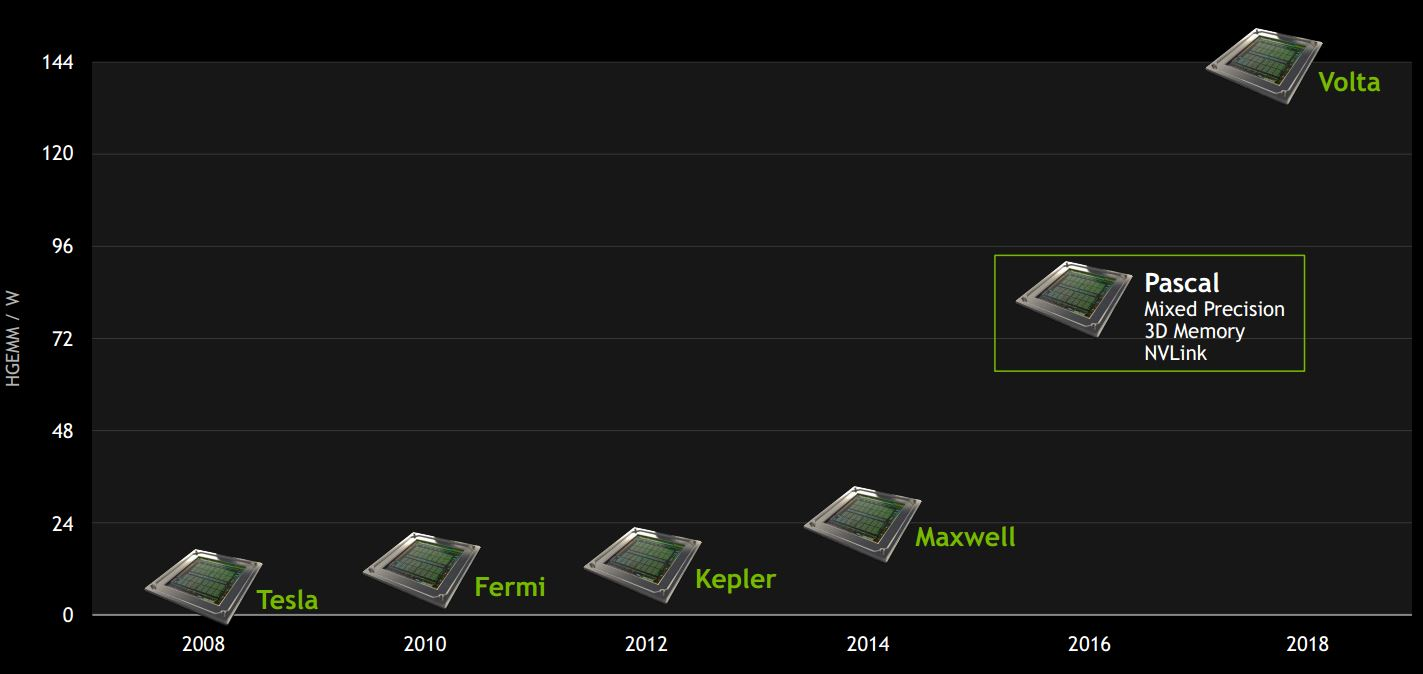
\includegraphics[scale=0.3]{GPU-Roadmap-GTC-2015-HGEMM}
\end{figure}
}

\frame{
\frametitle{Espaços de Memória em GPGPUs}
O acesso à memória global é custoso, a latência é $100x$ mais lenta que na memória compartilhada.
\begin{figure}[htpb]
 \centering
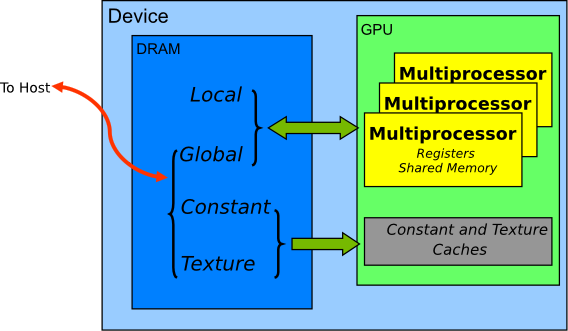
\includegraphics[scale=0.6]{memory-spaces-on-cuda-device}
\caption{Espaços de memória em dispositivos CUDA}
\end{figure}
}

\frame{
\frametitle{Compute Capability de GPUs NVIDIA}
Compute Capability é uma diferenciação entre arquiteturas e modelos de GPUs NVIDIA.
\begin{figure}[htpb]
 \centering
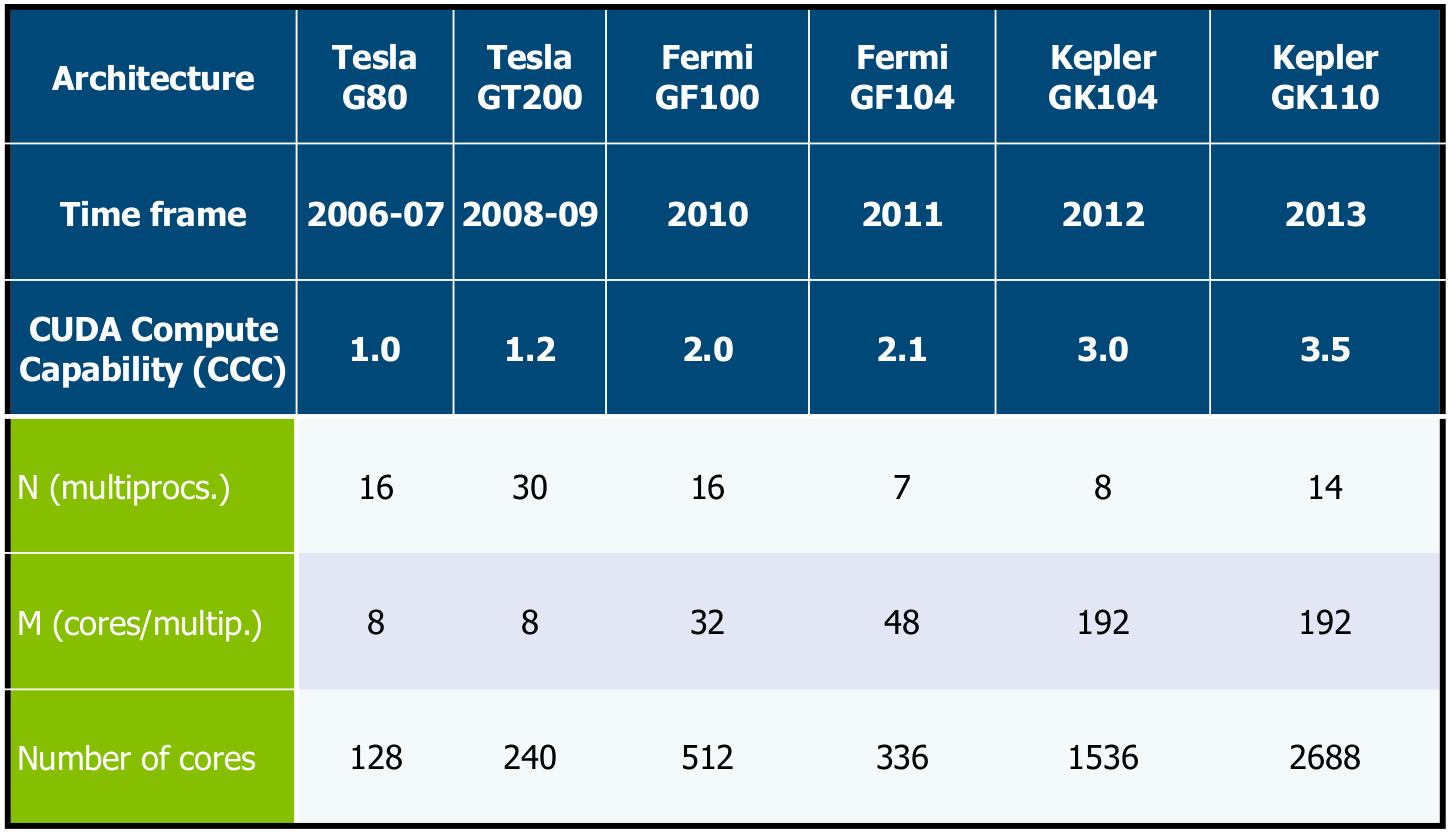
\includegraphics[scale=0.2]{gpuArchMap}
\end{figure}
}

\frame{
\frametitle{GPUs Tesla da NVIDIA}
\begin{minipage}{0.4\textwidth}
    \begin{itemize}
        \item Multiprocessadores
        \item FP 32
        \item FP 64
        \item Interface mem.
        \item TDP
        \item Fabricação
    \end{itemize}
\end{minipage}\hfill
\begin{minipage}{0.6\textwidth}
\begin{figure}[htpb]
 \centering
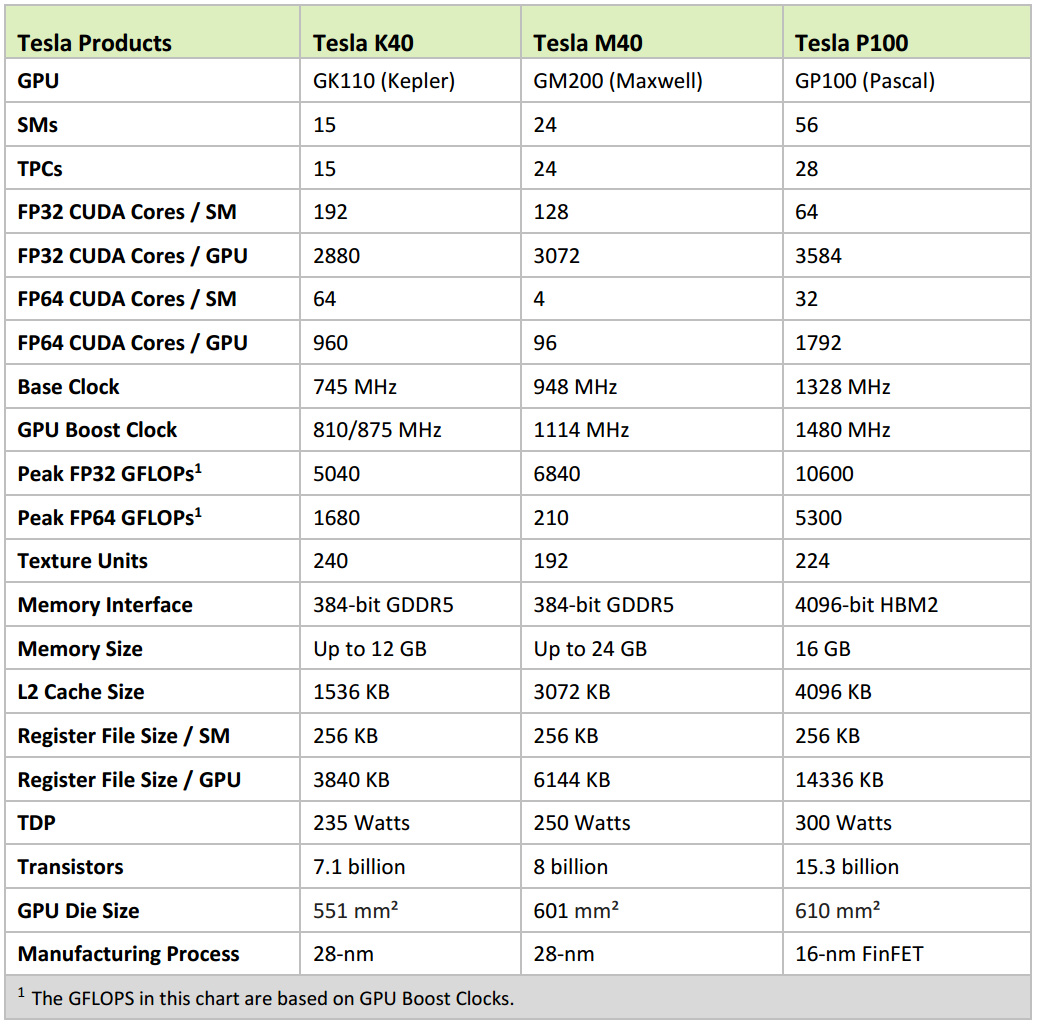
\includegraphics[scale=0.2]{Teslas-GPUs}
\label{fig:TeslasGPUs}
\end{figure}
\end{minipage}
}

\frame{
\frametitle{Arquitetura Tesla: Primeiras GPGPU}
\begin{figure}[htpb]
 \centering
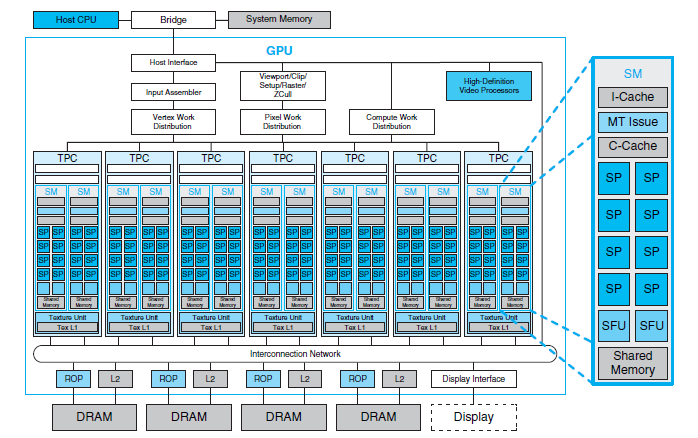
\includegraphics[scale=0.6]{Geforce-256-arch}
\label{fig:Teslaarch}
\end{figure}
}

\frame{
\frametitle{Multiprocessador da Arquitetura Fermi}
\scriptsize
\begin{minipage}{0.35\textwidth}
    \begin{itemize}
        \item Processo de fabricação 40 nm
        \item 16 Multiprocessadores
        \item 32 processadores
        \item 16 unidades leitura/escrita
        \item 4 unidades funções especiais
        \item 48 kB Memória compartilhada
        \item 32768 registradores
        \item 2 escalonadores de warps
    \end{itemize}
\end{minipage}\hfill
\begin{minipage}{0.65\textwidth}
\begin{figure}[htpb]
 \centering
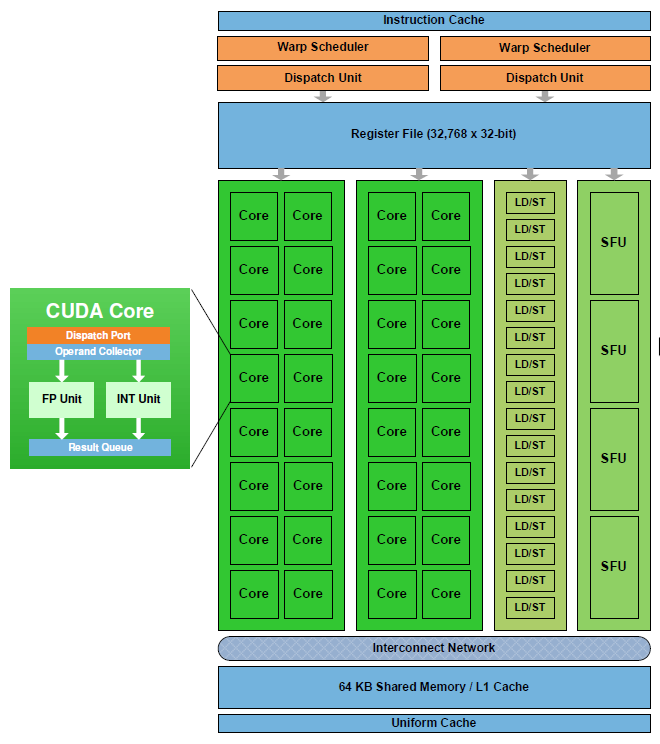
\includegraphics[scale=0.265]{fermi-sm}
\label{fig:FermiSM}
\end{figure}
\end{minipage}
}

\frame{
\frametitle{Arquitetura Fermi}
\begin{figure}[htpb]
 \centering
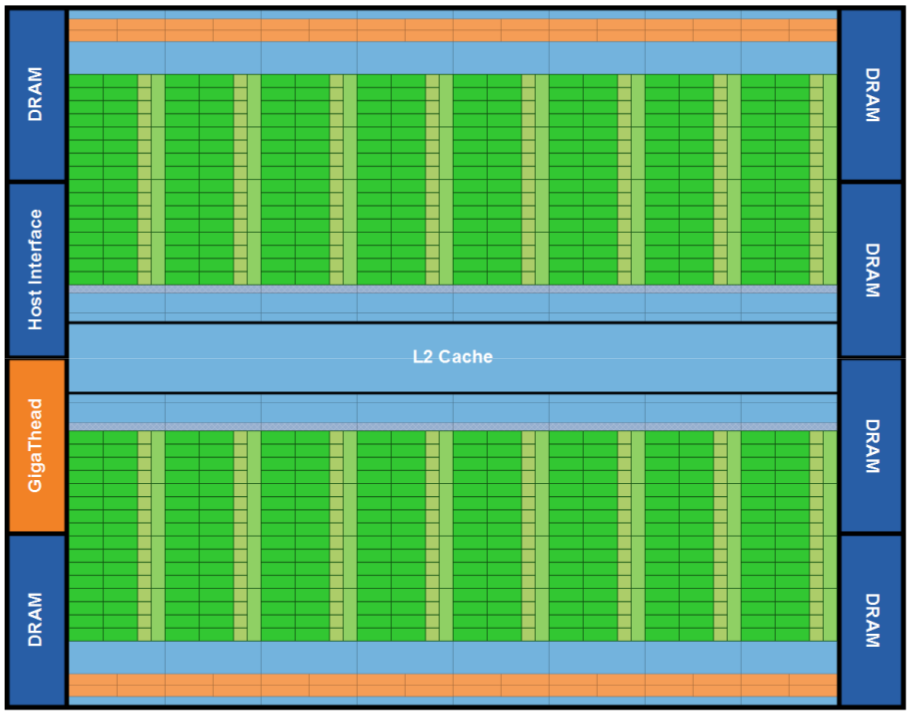
\includegraphics[scale=0.275]{fermi-arch}
\label{fig:Fermiarch}
\end{figure}
}

\frame{
\frametitle{Multiprocessador da Arquitetura Kepler}
\scriptsize
\begin{minipage}{0.35\textwidth}
    \begin{itemize}
        \item Processo de fabricação 28 nm
        \item 15 SMX de 192 cores
        \item 2880 CUDA Cores
        \item 64 KB do arquivo de registradores
        \item 3072 KB de cache L2
        \item Até 24 GB de memória GDDR5
        \item Hyper-Q
        \item Paralelismo dinâmico
        \item 4 escalonadores de warps
    \end{itemize}
\end{minipage}\hfill
\begin{minipage}{0.65\textwidth}
\begin{figure}[htpb]
 \centering
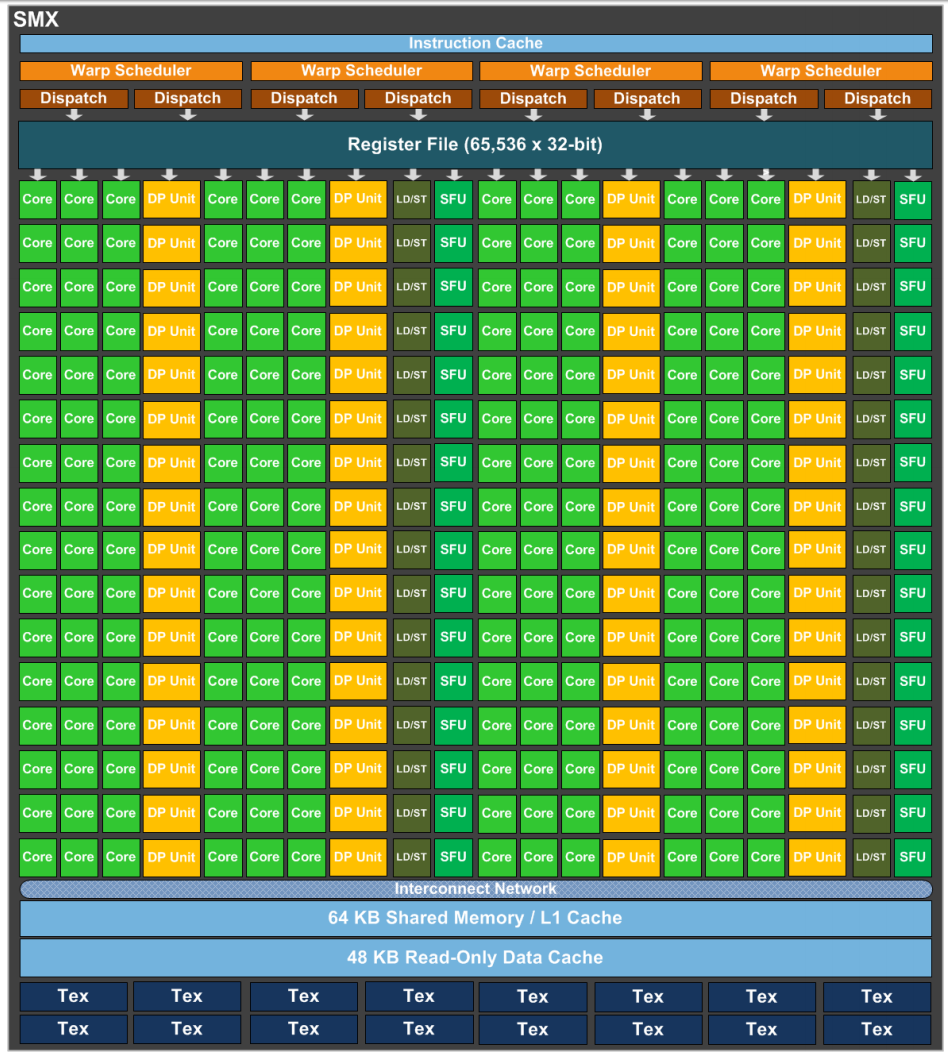
\includegraphics[scale=0.2]{kepler-smx}
\label{fig:keplerSM}
\end{figure}
\end{minipage}
}

\frame{
\frametitle{Arquitetura Kepler}
\begin{figure}[htpb]
 \centering
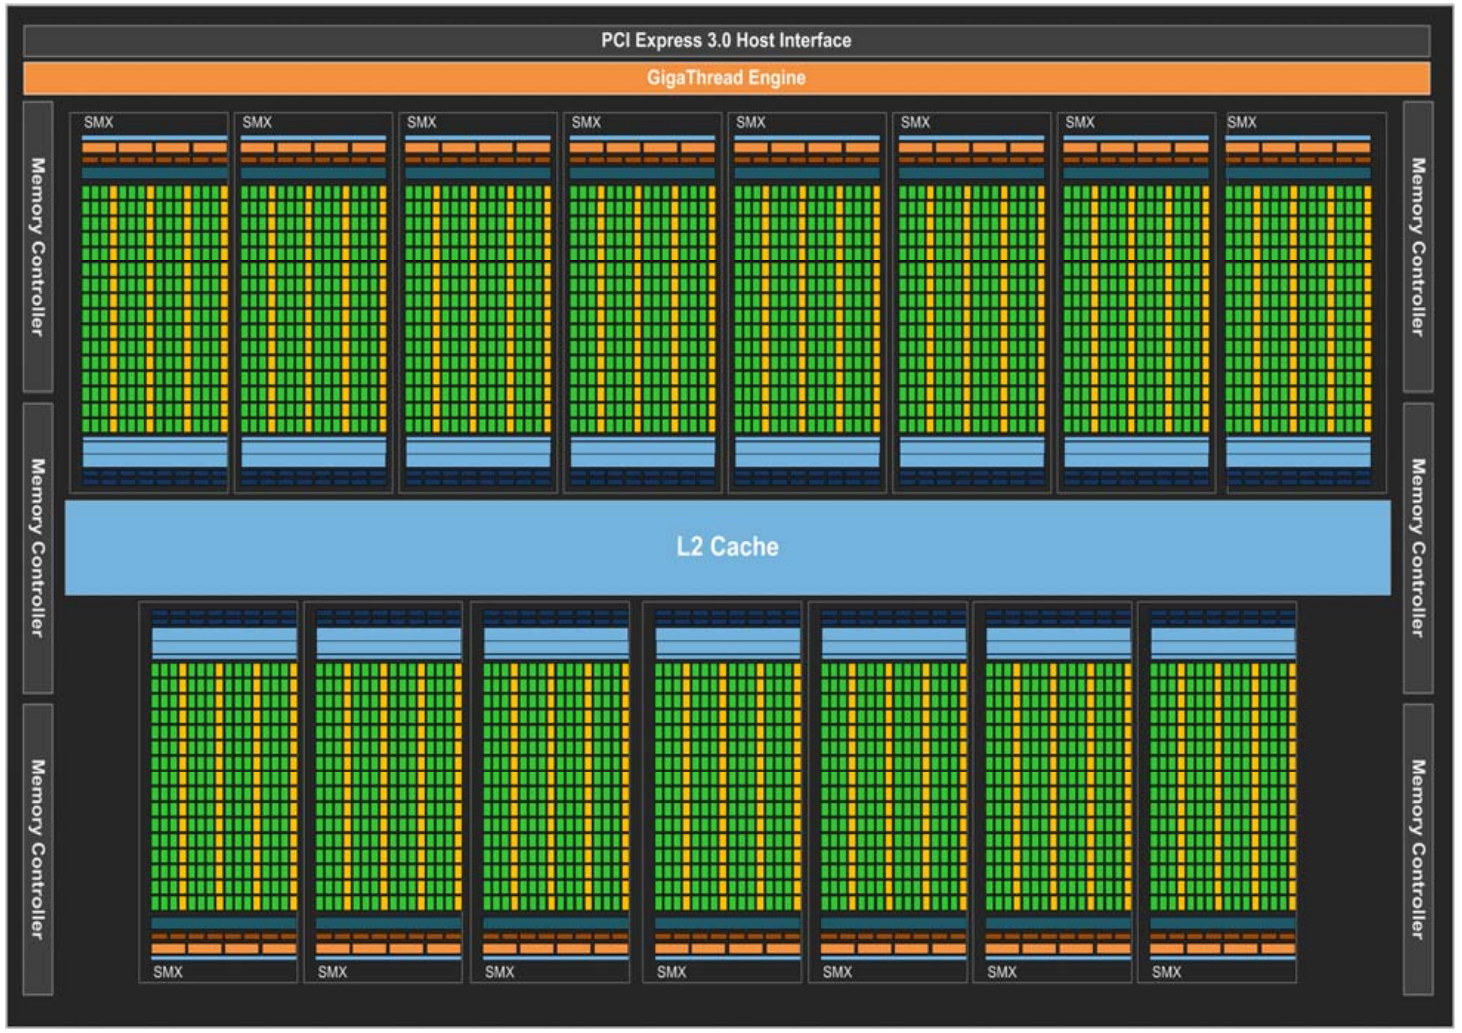
\includegraphics[scale=0.2]{kepler-gk110-arch}
\label{fig:keplerarch}
\end{figure}
}

\frame{
\frametitle{Multiprocessador da Arquitetura Maxwell}
\begin{minipage}{0.6\textwidth}
\scriptsize
    \begin{itemize}
        \item Cluster Processamento Gráfico-GPC
        \item 128 CUDA cores por SMM
        \item Dividido em 4 distintos 32 cores FP
        \item 96 KB de memória compartilhada dedicada
        \item 48 KB de cache L1/cache textura (unificado)        
        \item 2 MB  de memória cache L2
\end{itemize}
\end{minipage}\hfill
\begin{minipage}{0.4\textwidth}

\begin{figure}[htpb]
 \centering
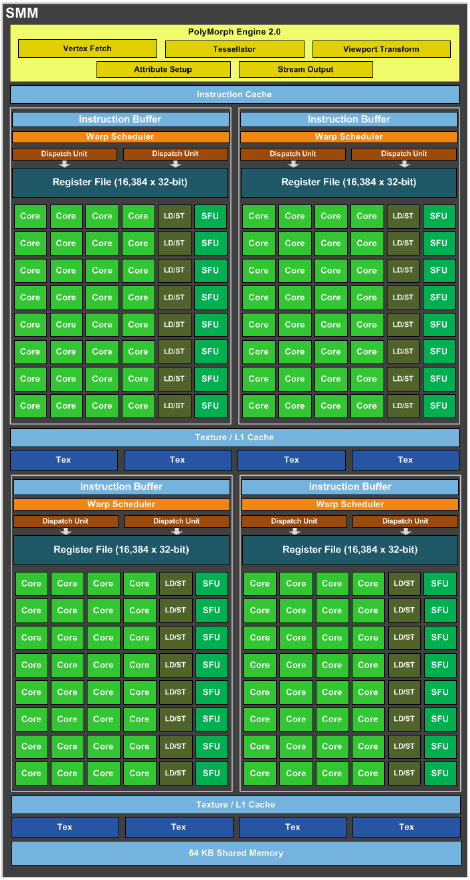
\includegraphics[scale=0.3]{maxwell-smm}
\label{fig:maxwellSMM}
\end{figure}
\end{minipage}
}

\frame{
\frametitle{Arquitetura Maxwell}
\begin{figure}[htpb]
 \centering
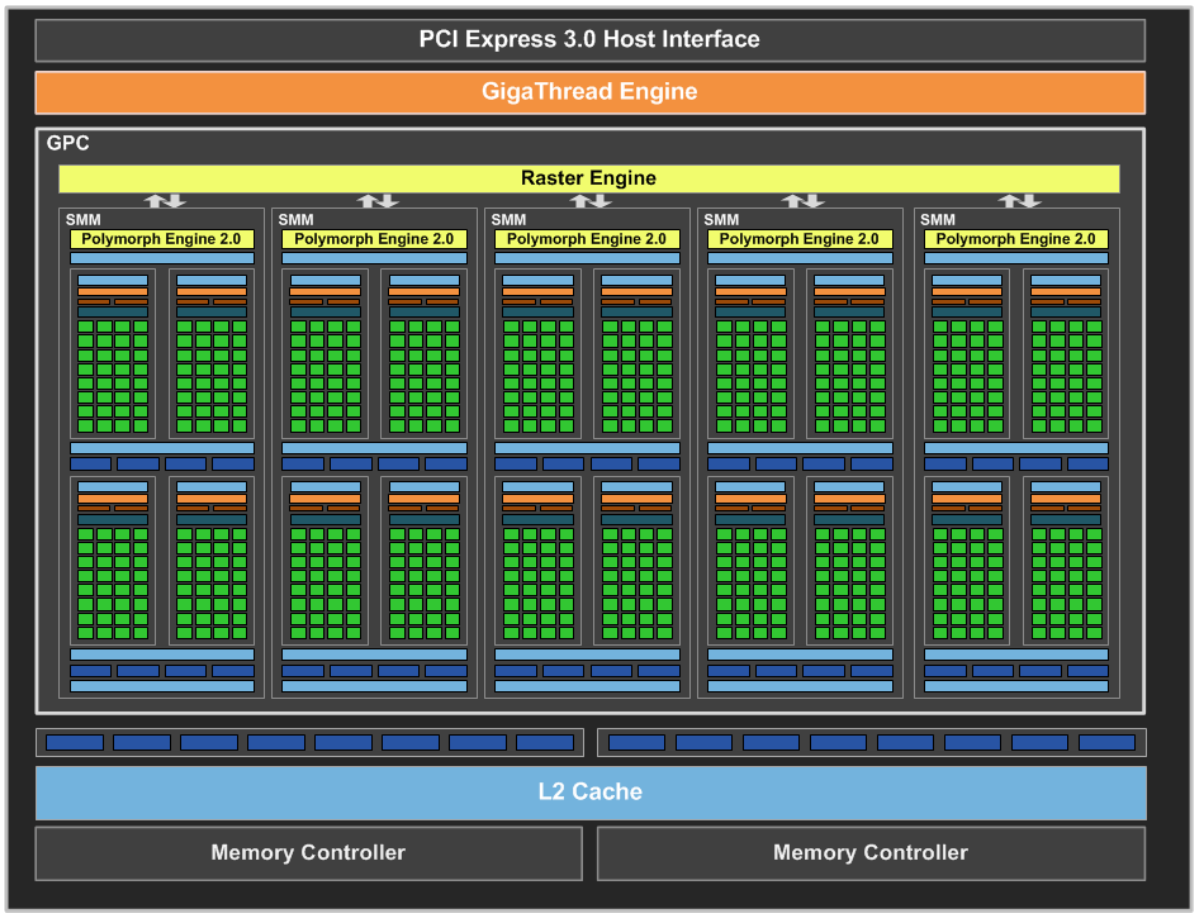
\includegraphics[scale=0.325]{maxwell-gpc}
\label{fig:maxwellarch}
\end{figure}
}


\frame{
\frametitle{Arquitetura Pascal}
    \begin{itemize}	
        \item Cada SM está dividido em 2 blocos de processamento
        \item SMs of 64 cores de precisão simples
        \item 32 unidades de precisão dupla  
        \item 64/2 KB de memória compartilhada dedicada
        \item 4096-bit na interface de memória
        \item HBM Stacked DRAM
        \item Preempção na computação
        \item NVLink        
    \end{itemize}
}


\frame{
\frametitle{Multiprocessador da Arquitetura Pascal}
\begin{figure}[htpb]
 \centering
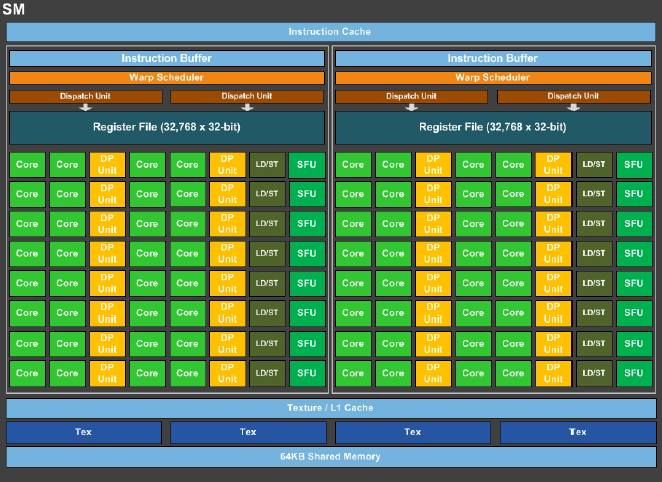
\includegraphics[scale=0.425]{pascal-sm}
\caption{Multiprocessador da arquitetura Pascal}
\label{fig:pascalSMM}
\end{figure}
}


\frame{
\frametitle{Arquitetura Pascal: NVLink}
\begin{figure}[htpb]
 \centering
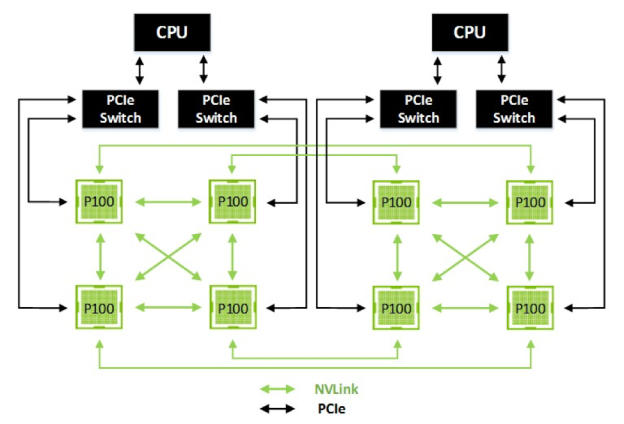
\includegraphics[scale=0.9]{Nvlink.png}
\caption{NVLink ligando 8 Tesla P100 em uma topologia Hibrida Cubo malha}
\label{fig:nvlink}
\end{figure}
}

\subsection{GPGPUs AMD}

\begin{frame}
    \frametitle{GPGPUs AMD}
    \begin{center}
        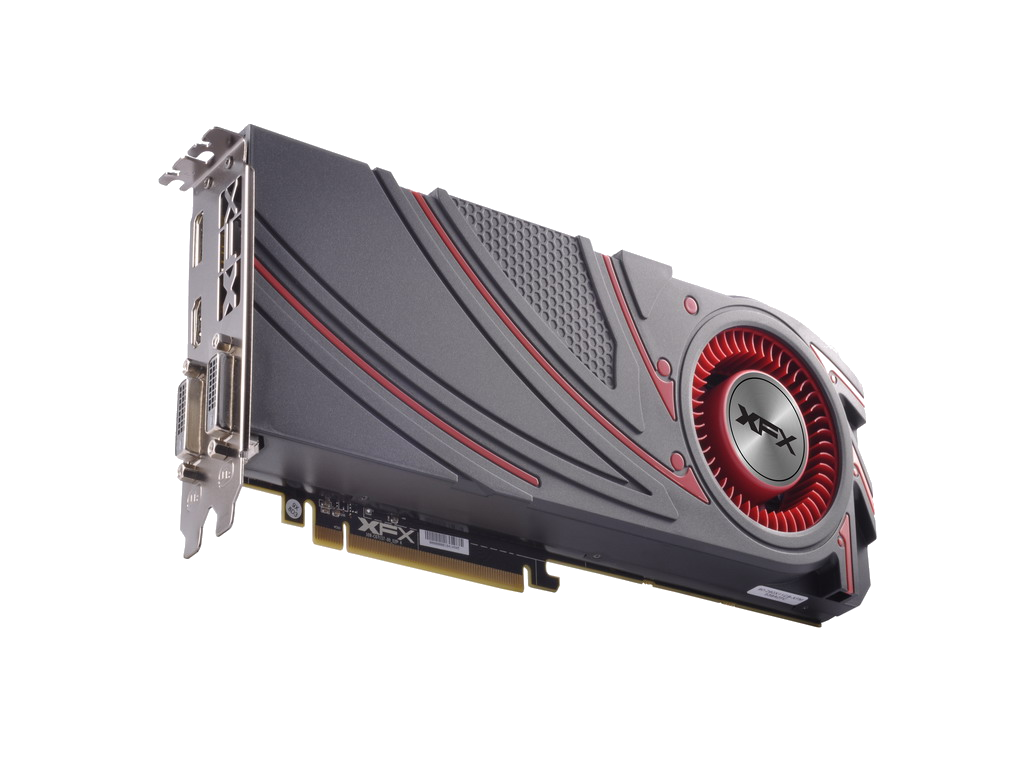
\includegraphics[width=\textwidth]{r9390p}
    \end{center}
\end{frame}

\frame{
\frametitle{GPUs de Próposito Geral da AMD}
Evolução das GPUs AMD:

\begin{itemize}
    \item Array Technology Inc. (ATI): 1985
    \item Visual Processing Unit (VPU), da ATI
    \item Advanced Micro Devices (AMD) adquire a ATI: 2006
    \item Graphic Core Next (GCN): 2011
    \item AMD Radeon HD 7790, usa GCN 1.1: 2012
    \item GCN: 5a. Geração
\end{itemize}
}

\frame{
    \frametitle{Graphic Core Next}
\begin{minipage}{0.475\textwidth}
    \begin{figure}[htpb]
        \centering
        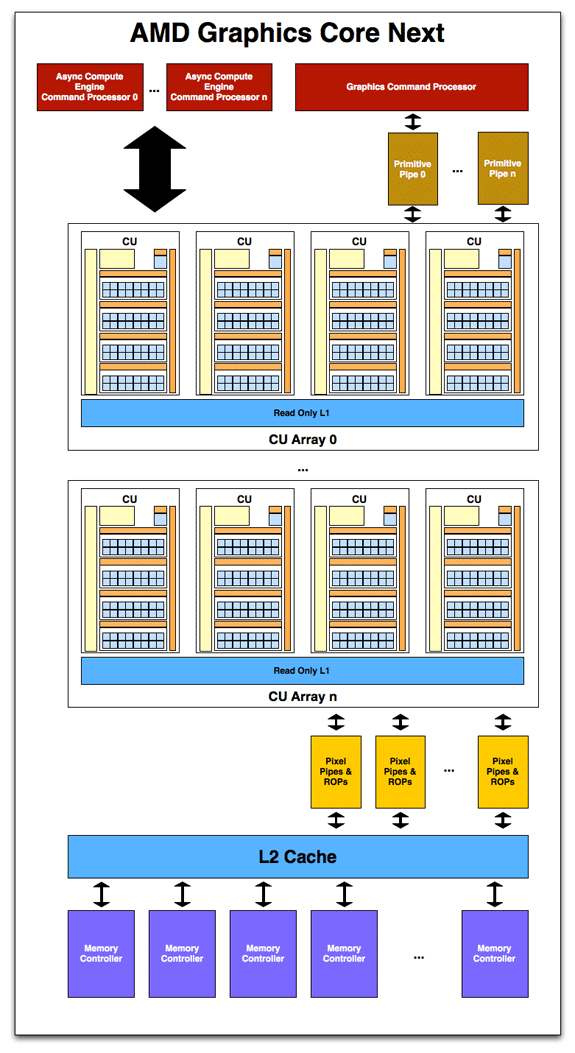
\includegraphics[scale=0.225]{AMD-GCN-3Th}
        \label{fig:AMD-GCN}
    \end{figure}
\end{minipage}\hfill
\begin{minipage}{0.475\textwidth}
    \begin{figure}[htpb]
        \centering
        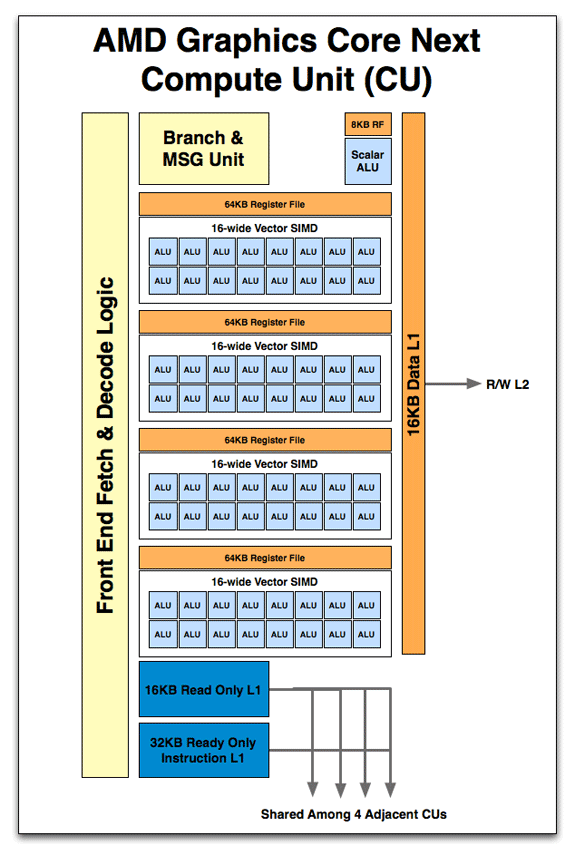
\includegraphics[scale=0.25]{Core-AMD-GCN}
        \label{fig:Core-AMD-GCN}
    \end{figure}
\end{minipage}
}

\frame{
\frametitle{Roadmap para as GPUs AMD}
\begin{figure}[htpb]
 \centering
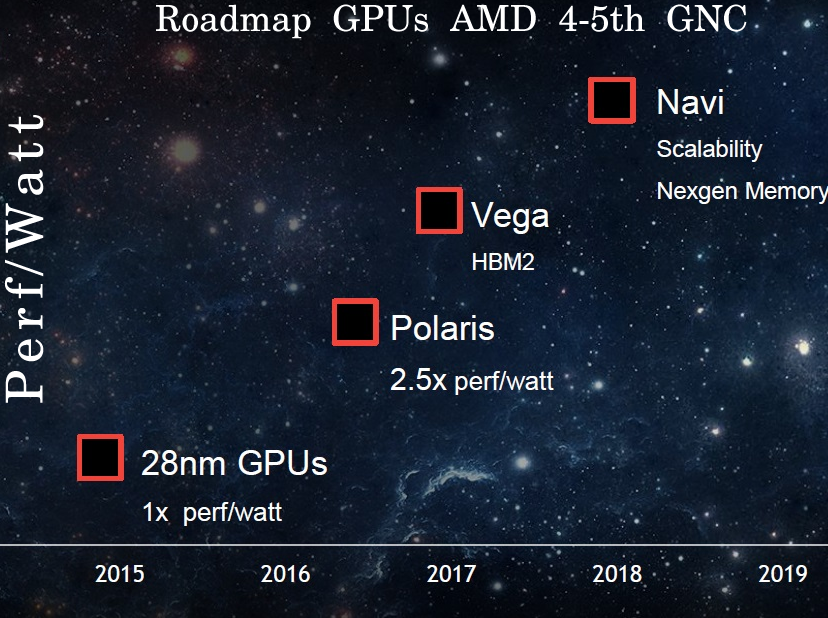
\includegraphics[scale=0.45]{AMDGPU}
\label{fig:roadmapAMD}
\end{figure}
}

\section{Intel Xeon Phi}

\begin{frame}
    \frametitle{Intel Xeon Phi}
    \begin{center}
        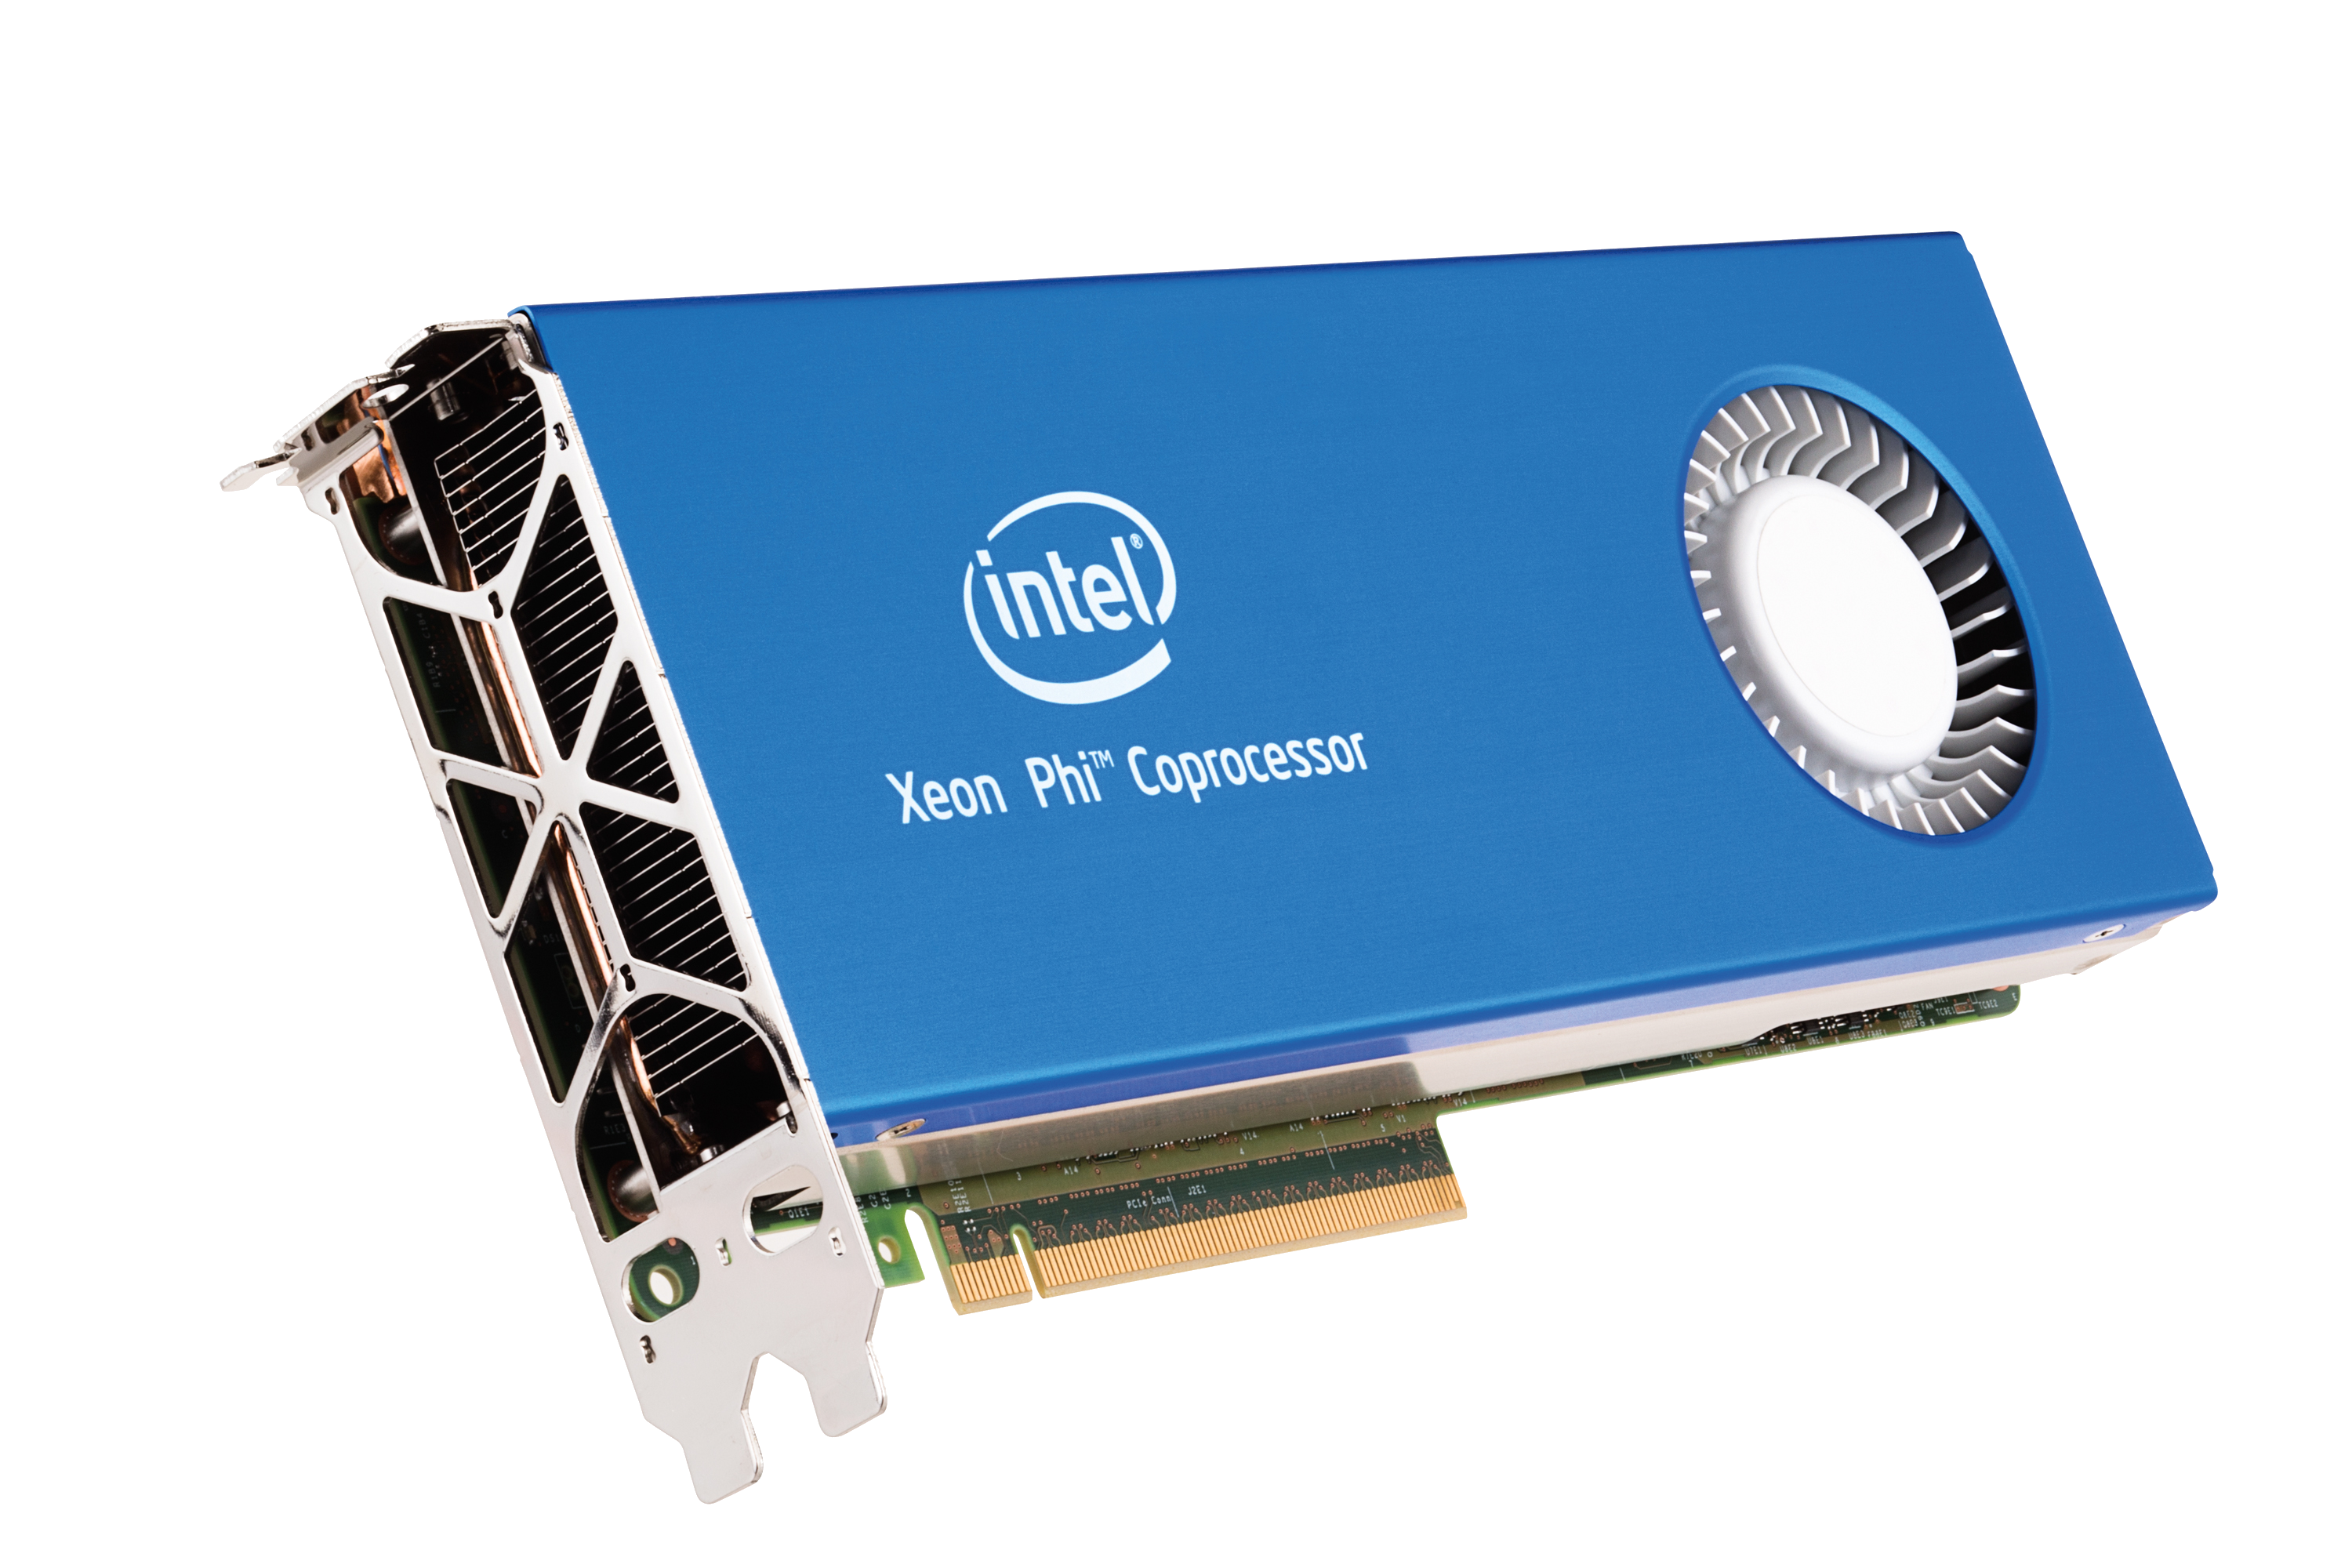
\includegraphics[width=\textwidth]{xeonphi}
    \end{center}
\end{frame}

\frame{
\frametitle{Roadmap para Intel Xeon Phi}
\begin{itemize}
\item Larrabee: 2006-2010 $\rightarrow$ Knights Ferry: 2010
\item 1$^a$. geração x100 Knights Corner: 22 nm
\item 2$^a$. geração x200 Knights Landing: 14 nm
\item 3$^a$. geração Knights Hill: 10 nm
\end{itemize}

\begin{figure}[h!]
\centering
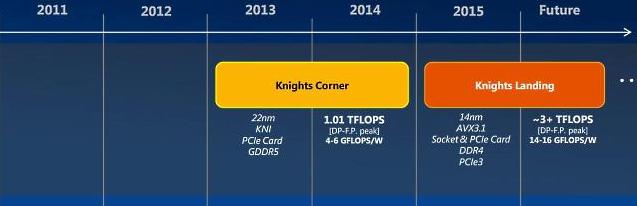
\includegraphics[scale=.65]{roadMapKnightIntel}
\label{fig:RMXeonphi}
\end{figure}
}

\frame{
\frametitle{Knights Corner: Arquitetura}
\begin{figure}[h!]
\centering
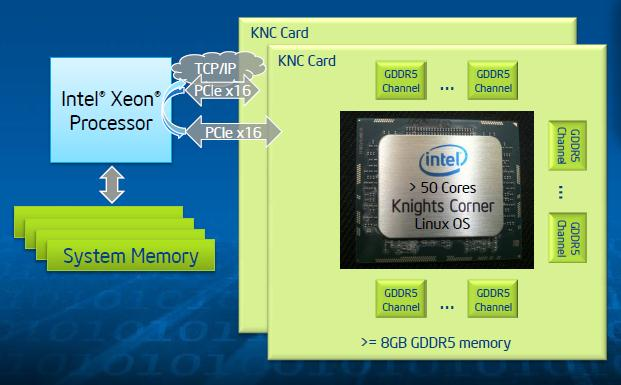
\includegraphics[scale=.475]{intelXeonPhi}
\label{fig:Xeonphi}
\end{figure}
}

\frame{
\frametitle{Anel de Interconexão Bidirecional}
\begin{figure}[h!]
\centering
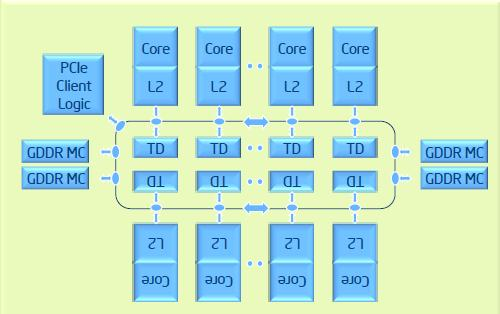
\includegraphics[scale=.6]{bidirectionalRingXeonPhi}
\label{fig:AnelBidireccional}
\end{figure}
}

\frame{
\frametitle{Core do Xeon Phi}
\begin{figure}[h!]
\centering
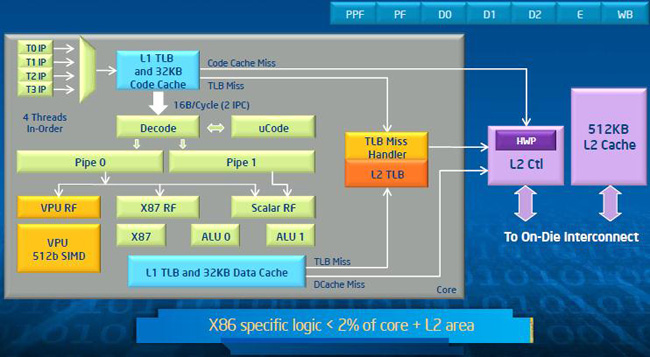
\includegraphics[scale=.475]{CoreXeonPhi}
\label{fig:coreXeonPhi}
\end{figure}
}

\frame{
\frametitle{Unidade de Processamento Vetorial}
\begin{figure}[h!]
\centering
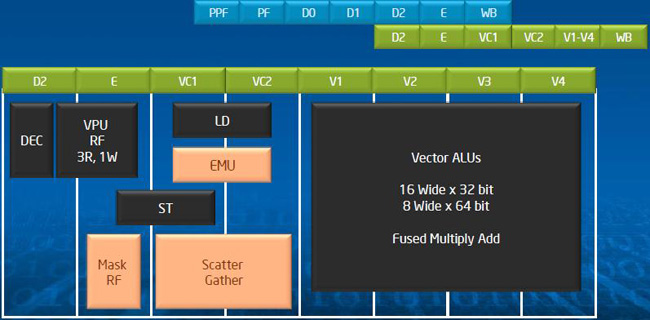
\includegraphics[scale=.475]{vectorProcessingUnitXeonPhi}
\label{fig:VPUXeonPhi}
\end{figure}
}

\frame{
\frametitle{Desempenho por Watts de alguns aceleradores}
\begin{figure}[h!]
\centering
\includegraphics[scale=.475]{PerfWattsXeonPhi}
\label{fig:PerfWattsXeonPhi}
\end{figure}
}

\frame{
\frametitle{Intel Parallel Studio}
\begin{figure}[h!]
\centering
\includegraphics[scale=.4]{Intel-VTune}
\caption{Intel Vtune Amplifier}
\label{fig:Vtune}
\end{figure}
}

\frame{
\frametitle{OpenACC}
OpenACC:
\begin{itemize}
    \item Padrão para Programação Paralela
    \item Baseado no compilador PGI (Portland Group)
    \item Fornece coleção de diretivas para especificar laços e regiões de
        código paralelizáveis
\end{itemize}

\begin{figure}[htpd]
\centering
\includegraphics[scale=.4]{accelerators}
\end{figure}
}

\maketitle

\end{document}
